\documentclass{article}
% The [final] option alone leaves the track name undefined; supply the main-track footer text.
\makeatletter\providecommand{\@trackname}{39th Conference on Neural Information Processing Systems (NeurIPS 2025).}\makeatother
\usepackage[final]{neurips_2025}  % NEURIPS style (neurips_2025.sty is in paper_draft/)
\usepackage[hidelinks]{hyperref}  % REQUIRED: clickable links
\usepackage{booktabs}  % REQUIRED: professional tables
\usepackage{graphicx}
\usepackage{amsmath,amssymb}

\usepackage[utf8]{inputenc}
\usepackage[T1]{fontenc}
\usepackage{xspace}
\usepackage{enumitem}
\usepackage{subcaption}
\usepackage{multirow}
\usepackage{makecell}
\usepackage{tikz}
\usetikzlibrary{arrows.meta,positioning,fit,calc}
\usepackage{algorithm}
\usepackage[noend]{algpseudocode}

% Import command files
%%%%% MATH NOTATION MACROS %%%%%
% Standard math notation for academic papers
% Import with: %%%%% MATH NOTATION MACROS %%%%%
% Standard math notation for academic papers
% Import with: %%%%% MATH NOTATION MACROS %%%%%
% Standard math notation for academic papers
% Import with: \input{commands/math}

\usepackage{amsmath,amsfonts,bm}

%%%%%%%%%%%%%%%%%%%%%%%%%%%%%%%%%%%%%%%%%%%%%%%%%%%%%%%%%%%%%%%%%
% FIGURE AND SECTION REFERENCES
%%%%%%%%%%%%%%%%%%%%%%%%%%%%%%%%%%%%%%%%%%%%%%%%%%%%%%%%%%%%%%%%%

% Mark sections of captions for referring to divisions of figures
\newcommand{\figleft}{{\em (Left)}}
\newcommand{\figcenter}{{\em (Center)}}
\newcommand{\figright}{{\em (Right)}}
\newcommand{\figtop}{{\em (Top)}}
\newcommand{\figbottom}{{\em (Bottom)}}
\newcommand{\captiona}{{\em (a)}}
\newcommand{\captionb}{{\em (b)}}
\newcommand{\captionc}{{\em (c)}}
\newcommand{\captiond}{{\em (d)}}

% Figure references
\def\figref#1{figure~\ref{#1}}
\def\Figref#1{Figure~\ref{#1}}
\def\twofigref#1#2{figures \ref{#1} and \ref{#2}}
\def\quadfigref#1#2#3#4{figures \ref{#1}, \ref{#2}, \ref{#3} and \ref{#4}}

% Section references
\def\secref#1{section~\ref{#1}}
\def\Secref#1{Section~\ref{#1}}
\def\twosecrefs#1#2{sections \ref{#1} and \ref{#2}}
\def\secrefs#1#2#3{sections \ref{#1}, \ref{#2} and \ref{#3}}

% Equation references
\def\eqref#1{equation~\ref{#1}}
\def\Eqref#1{Equation~\ref{#1}}
\def\plaineqref#1{\ref{#1}}

% Algorithm references
\def\algref#1{algorithm~\ref{#1}}
\def\Algref#1{Algorithm~\ref{#1}}
\def\twoalgref#1#2{algorithms \ref{#1} and \ref{#2}}
\def\Twoalgref#1#2{Algorithms \ref{#1} and \ref{#2}}

% Table references
\def\tabref#1{table~\ref{#1}}
\def\Tabref#1{Table~\ref{#1}}

% Chapter references
\def\chapref#1{chapter~\ref{#1}}
\def\Chapref#1{Chapter~\ref{#1}}

%%%%%%%%%%%%%%%%%%%%%%%%%%%%%%%%%%%%%%%%%%%%%%%%%%%%%%%%%%%%%%%%%
% BASIC MATH DEFINITIONS
%%%%%%%%%%%%%%%%%%%%%%%%%%%%%%%%%%%%%%%%%%%%%%%%%%%%%%%%%%%%%%%%%

\def\ceil#1{\lceil #1 \rceil}
\def\floor#1{\lfloor #1 \rfloor}
\def\1{\bm{1}}
\def\eps{{\epsilon}}

% Common operators
\DeclareMathOperator*{\argmax}{arg\,max}
\DeclareMathOperator*{\argmin}{arg\,min}
\DeclareMathOperator{\sign}{sign}
\DeclareMathOperator{\Tr}{Tr}
\let\ab\allowbreak

%%%%%%%%%%%%%%%%%%%%%%%%%%%%%%%%%%%%%%%%%%%%%%%%%%%%%%%%%%%%%%%%%
% VECTORS (lowercase bold)
%%%%%%%%%%%%%%%%%%%%%%%%%%%%%%%%%%%%%%%%%%%%%%%%%%%%%%%%%%%%%%%%%

\def\vzero{{\bm{0}}}
\def\vone{{\bm{1}}}
\def\vmu{{\bm{\mu}}}
\def\vtheta{{\bm{\theta}}}
\def\va{{\bm{a}}}
\def\vb{{\bm{b}}}
\def\vc{{\bm{c}}}
\def\vd{{\bm{d}}}
\def\ve{{\bm{e}}}
\def\vf{{\bm{f}}}
\def\vg{{\bm{g}}}
\def\vh{{\bm{h}}}
\def\vi{{\bm{i}}}
\def\vj{{\bm{j}}}
\def\vk{{\bm{k}}}
\def\vl{{\bm{l}}}
\def\vm{{\bm{m}}}
\def\vn{{\bm{n}}}
\def\vo{{\bm{o}}}
\def\vp{{\bm{p}}}
\def\vq{{\bm{q}}}
\def\vr{{\bm{r}}}
\def\vs{{\bm{s}}}
\def\vt{{\bm{t}}}
\def\vu{{\bm{u}}}
\def\vv{{\bm{v}}}
\def\vw{{\bm{w}}}
\def\vx{{\bm{x}}}
\def\vy{{\bm{y}}}
\def\vz{{\bm{z}}}

%%%%%%%%%%%%%%%%%%%%%%%%%%%%%%%%%%%%%%%%%%%%%%%%%%%%%%%%%%%%%%%%%
% MATRICES (uppercase bold)
%%%%%%%%%%%%%%%%%%%%%%%%%%%%%%%%%%%%%%%%%%%%%%%%%%%%%%%%%%%%%%%%%

\def\mA{{\bm{A}}}
\def\mB{{\bm{B}}}
\def\mC{{\bm{C}}}
\def\mD{{\bm{D}}}
\def\mE{{\bm{E}}}
\def\mF{{\bm{F}}}
\def\mG{{\bm{G}}}
\def\mH{{\bm{H}}}
\def\mI{{\bm{I}}}
\def\mJ{{\bm{J}}}
\def\mK{{\bm{K}}}
\def\mL{{\bm{L}}}
\def\mM{{\bm{M}}}
\def\mN{{\bm{N}}}
\def\mO{{\bm{O}}}
\def\mP{{\bm{P}}}
\def\mQ{{\bm{Q}}}
\def\mR{{\bm{R}}}
\def\mS{{\bm{S}}}
\def\mT{{\bm{T}}}
\def\mU{{\bm{U}}}
\def\mV{{\bm{V}}}
\def\mW{{\bm{W}}}
\def\mX{{\bm{X}}}
\def\mY{{\bm{Y}}}
\def\mZ{{\bm{Z}}}
\def\mBeta{{\bm{\beta}}}
\def\mPhi{{\bm{\Phi}}}
\def\mLambda{{\bm{\Lambda}}}
\def\mSigma{{\bm{\Sigma}}}

%%%%%%%%%%%%%%%%%%%%%%%%%%%%%%%%%%%%%%%%%%%%%%%%%%%%%%%%%%%%%%%%%
% CALLIGRAPHIC (mathcal)
%%%%%%%%%%%%%%%%%%%%%%%%%%%%%%%%%%%%%%%%%%%%%%%%%%%%%%%%%%%%%%%%%

\def\gA{{\mathcal{A}}}
\def\gB{{\mathcal{B}}}
\def\gC{{\mathcal{C}}}
\def\gD{{\mathcal{D}}}
\def\gE{{\mathcal{E}}}
\def\gF{{\mathcal{F}}}
\def\gG{{\mathcal{G}}}
\def\gH{{\mathcal{H}}}
\def\gI{{\mathcal{I}}}
\def\gJ{{\mathcal{J}}}
\def\gK{{\mathcal{K}}}
\def\gL{{\mathcal{L}}}
\def\gM{{\mathcal{M}}}
\def\gN{{\mathcal{N}}}
\def\gO{{\mathcal{O}}}
\def\gP{{\mathcal{P}}}
\def\gQ{{\mathcal{Q}}}
\def\gR{{\mathcal{R}}}
\def\gS{{\mathcal{S}}}
\def\gT{{\mathcal{T}}}
\def\gU{{\mathcal{U}}}
\def\gV{{\mathcal{V}}}
\def\gW{{\mathcal{W}}}
\def\gX{{\mathcal{X}}}
\def\gY{{\mathcal{Y}}}
\def\gZ{{\mathcal{Z}}}

%%%%%%%%%%%%%%%%%%%%%%%%%%%%%%%%%%%%%%%%%%%%%%%%%%%%%%%%%%%%%%%%%
% SETS (blackboard bold)
%%%%%%%%%%%%%%%%%%%%%%%%%%%%%%%%%%%%%%%%%%%%%%%%%%%%%%%%%%%%%%%%%

\def\sA{{\mathbb{A}}}
\def\sB{{\mathbb{B}}}
\def\sC{{\mathbb{C}}}
\def\sD{{\mathbb{D}}}
\def\sF{{\mathbb{F}}}
\def\sG{{\mathbb{G}}}
\def\sH{{\mathbb{H}}}
\def\sI{{\mathbb{I}}}
\def\sJ{{\mathbb{J}}}
\def\sK{{\mathbb{K}}}
\def\sL{{\mathbb{L}}}
\def\sM{{\mathbb{M}}}
\def\sN{{\mathbb{N}}}
\def\sO{{\mathbb{O}}}
\def\sP{{\mathbb{P}}}
\def\sQ{{\mathbb{Q}}}
\def\sR{{\mathbb{R}}}
\def\sS{{\mathbb{S}}}
\def\sT{{\mathbb{T}}}
\def\sU{{\mathbb{U}}}
\def\sV{{\mathbb{V}}}
\def\sW{{\mathbb{W}}}
\def\sX{{\mathbb{X}}}
\def\sY{{\mathbb{Y}}}
\def\sZ{{\mathbb{Z}}}

%%%%%%%%%%%%%%%%%%%%%%%%%%%%%%%%%%%%%%%%%%%%%%%%%%%%%%%%%%%%%%%%%
% COMMON MATH SHORTCUTS
%%%%%%%%%%%%%%%%%%%%%%%%%%%%%%%%%%%%%%%%%%%%%%%%%%%%%%%%%%%%%%%%%

% Expectation and variance
\newcommand{\E}{\mathbb{E}}
\newcommand{\Var}{\mathrm{Var}}
\newcommand{\Cov}{\mathrm{Cov}}
\newcommand{\R}{\mathbb{R}}

% Datasets
\newcommand{\train}{\mathcal{D}}
\newcommand{\valid}{\mathcal{D_{\mathrm{valid}}}}
\newcommand{\test}{\mathcal{D_{\mathrm{test}}}}

% Distributions
\newcommand{\laplace}{\mathrm{Laplace}}
\newcommand{\Uniform}{\mathrm{Unif}}
\newcommand{\Normal}{\mathrm{Normal}}
\newcommand{\Categorical}{\mathrm{Categorical}}

% Common functions
\newcommand{\softmax}{\mathrm{softmax}}
\newcommand{\sigmoid}{\sigma}
\newcommand{\KL}{D_{\mathrm{KL}}}

% Norms
\newcommand{\normlzero}{L^0}
\newcommand{\normlone}{L^1}
\newcommand{\normltwo}{L^2}
\newcommand{\normlp}{L^p}
\newcommand{\normmax}{L^\infty}

%%%%%%%%%%%%%%%%%%%%%%%%%%%%%%%%%%%%%%%%%%%%%%%%%%%%%%%%%%%%%%%%%
% DEFINITIONS AND HIGHLIGHTING
%%%%%%%%%%%%%%%%%%%%%%%%%%%%%%%%%%%%%%%%%%%%%%%%%%%%%%%%%%%%%%%%%

% Highlight a newly defined term
\newcommand{\newterm}[1]{{\bf #1}}
\newcommand{\defn}[1]{\textbf{#1}}
\newcommand{\defeq}{\mathrel{\stackrel{\textnormal{\tiny def}}{=}}}


\usepackage{amsmath,amsfonts,bm}

%%%%%%%%%%%%%%%%%%%%%%%%%%%%%%%%%%%%%%%%%%%%%%%%%%%%%%%%%%%%%%%%%
% FIGURE AND SECTION REFERENCES
%%%%%%%%%%%%%%%%%%%%%%%%%%%%%%%%%%%%%%%%%%%%%%%%%%%%%%%%%%%%%%%%%

% Mark sections of captions for referring to divisions of figures
\newcommand{\figleft}{{\em (Left)}}
\newcommand{\figcenter}{{\em (Center)}}
\newcommand{\figright}{{\em (Right)}}
\newcommand{\figtop}{{\em (Top)}}
\newcommand{\figbottom}{{\em (Bottom)}}
\newcommand{\captiona}{{\em (a)}}
\newcommand{\captionb}{{\em (b)}}
\newcommand{\captionc}{{\em (c)}}
\newcommand{\captiond}{{\em (d)}}

% Figure references
\def\figref#1{figure~\ref{#1}}
\def\Figref#1{Figure~\ref{#1}}
\def\twofigref#1#2{figures \ref{#1} and \ref{#2}}
\def\quadfigref#1#2#3#4{figures \ref{#1}, \ref{#2}, \ref{#3} and \ref{#4}}

% Section references
\def\secref#1{section~\ref{#1}}
\def\Secref#1{Section~\ref{#1}}
\def\twosecrefs#1#2{sections \ref{#1} and \ref{#2}}
\def\secrefs#1#2#3{sections \ref{#1}, \ref{#2} and \ref{#3}}

% Equation references
\def\eqref#1{equation~\ref{#1}}
\def\Eqref#1{Equation~\ref{#1}}
\def\plaineqref#1{\ref{#1}}

% Algorithm references
\def\algref#1{algorithm~\ref{#1}}
\def\Algref#1{Algorithm~\ref{#1}}
\def\twoalgref#1#2{algorithms \ref{#1} and \ref{#2}}
\def\Twoalgref#1#2{Algorithms \ref{#1} and \ref{#2}}

% Table references
\def\tabref#1{table~\ref{#1}}
\def\Tabref#1{Table~\ref{#1}}

% Chapter references
\def\chapref#1{chapter~\ref{#1}}
\def\Chapref#1{Chapter~\ref{#1}}

%%%%%%%%%%%%%%%%%%%%%%%%%%%%%%%%%%%%%%%%%%%%%%%%%%%%%%%%%%%%%%%%%
% BASIC MATH DEFINITIONS
%%%%%%%%%%%%%%%%%%%%%%%%%%%%%%%%%%%%%%%%%%%%%%%%%%%%%%%%%%%%%%%%%

\def\ceil#1{\lceil #1 \rceil}
\def\floor#1{\lfloor #1 \rfloor}
\def\1{\bm{1}}
\def\eps{{\epsilon}}

% Common operators
\DeclareMathOperator*{\argmax}{arg\,max}
\DeclareMathOperator*{\argmin}{arg\,min}
\DeclareMathOperator{\sign}{sign}
\DeclareMathOperator{\Tr}{Tr}
\let\ab\allowbreak

%%%%%%%%%%%%%%%%%%%%%%%%%%%%%%%%%%%%%%%%%%%%%%%%%%%%%%%%%%%%%%%%%
% VECTORS (lowercase bold)
%%%%%%%%%%%%%%%%%%%%%%%%%%%%%%%%%%%%%%%%%%%%%%%%%%%%%%%%%%%%%%%%%

\def\vzero{{\bm{0}}}
\def\vone{{\bm{1}}}
\def\vmu{{\bm{\mu}}}
\def\vtheta{{\bm{\theta}}}
\def\va{{\bm{a}}}
\def\vb{{\bm{b}}}
\def\vc{{\bm{c}}}
\def\vd{{\bm{d}}}
\def\ve{{\bm{e}}}
\def\vf{{\bm{f}}}
\def\vg{{\bm{g}}}
\def\vh{{\bm{h}}}
\def\vi{{\bm{i}}}
\def\vj{{\bm{j}}}
\def\vk{{\bm{k}}}
\def\vl{{\bm{l}}}
\def\vm{{\bm{m}}}
\def\vn{{\bm{n}}}
\def\vo{{\bm{o}}}
\def\vp{{\bm{p}}}
\def\vq{{\bm{q}}}
\def\vr{{\bm{r}}}
\def\vs{{\bm{s}}}
\def\vt{{\bm{t}}}
\def\vu{{\bm{u}}}
\def\vv{{\bm{v}}}
\def\vw{{\bm{w}}}
\def\vx{{\bm{x}}}
\def\vy{{\bm{y}}}
\def\vz{{\bm{z}}}

%%%%%%%%%%%%%%%%%%%%%%%%%%%%%%%%%%%%%%%%%%%%%%%%%%%%%%%%%%%%%%%%%
% MATRICES (uppercase bold)
%%%%%%%%%%%%%%%%%%%%%%%%%%%%%%%%%%%%%%%%%%%%%%%%%%%%%%%%%%%%%%%%%

\def\mA{{\bm{A}}}
\def\mB{{\bm{B}}}
\def\mC{{\bm{C}}}
\def\mD{{\bm{D}}}
\def\mE{{\bm{E}}}
\def\mF{{\bm{F}}}
\def\mG{{\bm{G}}}
\def\mH{{\bm{H}}}
\def\mI{{\bm{I}}}
\def\mJ{{\bm{J}}}
\def\mK{{\bm{K}}}
\def\mL{{\bm{L}}}
\def\mM{{\bm{M}}}
\def\mN{{\bm{N}}}
\def\mO{{\bm{O}}}
\def\mP{{\bm{P}}}
\def\mQ{{\bm{Q}}}
\def\mR{{\bm{R}}}
\def\mS{{\bm{S}}}
\def\mT{{\bm{T}}}
\def\mU{{\bm{U}}}
\def\mV{{\bm{V}}}
\def\mW{{\bm{W}}}
\def\mX{{\bm{X}}}
\def\mY{{\bm{Y}}}
\def\mZ{{\bm{Z}}}
\def\mBeta{{\bm{\beta}}}
\def\mPhi{{\bm{\Phi}}}
\def\mLambda{{\bm{\Lambda}}}
\def\mSigma{{\bm{\Sigma}}}

%%%%%%%%%%%%%%%%%%%%%%%%%%%%%%%%%%%%%%%%%%%%%%%%%%%%%%%%%%%%%%%%%
% CALLIGRAPHIC (mathcal)
%%%%%%%%%%%%%%%%%%%%%%%%%%%%%%%%%%%%%%%%%%%%%%%%%%%%%%%%%%%%%%%%%

\def\gA{{\mathcal{A}}}
\def\gB{{\mathcal{B}}}
\def\gC{{\mathcal{C}}}
\def\gD{{\mathcal{D}}}
\def\gE{{\mathcal{E}}}
\def\gF{{\mathcal{F}}}
\def\gG{{\mathcal{G}}}
\def\gH{{\mathcal{H}}}
\def\gI{{\mathcal{I}}}
\def\gJ{{\mathcal{J}}}
\def\gK{{\mathcal{K}}}
\def\gL{{\mathcal{L}}}
\def\gM{{\mathcal{M}}}
\def\gN{{\mathcal{N}}}
\def\gO{{\mathcal{O}}}
\def\gP{{\mathcal{P}}}
\def\gQ{{\mathcal{Q}}}
\def\gR{{\mathcal{R}}}
\def\gS{{\mathcal{S}}}
\def\gT{{\mathcal{T}}}
\def\gU{{\mathcal{U}}}
\def\gV{{\mathcal{V}}}
\def\gW{{\mathcal{W}}}
\def\gX{{\mathcal{X}}}
\def\gY{{\mathcal{Y}}}
\def\gZ{{\mathcal{Z}}}

%%%%%%%%%%%%%%%%%%%%%%%%%%%%%%%%%%%%%%%%%%%%%%%%%%%%%%%%%%%%%%%%%
% SETS (blackboard bold)
%%%%%%%%%%%%%%%%%%%%%%%%%%%%%%%%%%%%%%%%%%%%%%%%%%%%%%%%%%%%%%%%%

\def\sA{{\mathbb{A}}}
\def\sB{{\mathbb{B}}}
\def\sC{{\mathbb{C}}}
\def\sD{{\mathbb{D}}}
\def\sF{{\mathbb{F}}}
\def\sG{{\mathbb{G}}}
\def\sH{{\mathbb{H}}}
\def\sI{{\mathbb{I}}}
\def\sJ{{\mathbb{J}}}
\def\sK{{\mathbb{K}}}
\def\sL{{\mathbb{L}}}
\def\sM{{\mathbb{M}}}
\def\sN{{\mathbb{N}}}
\def\sO{{\mathbb{O}}}
\def\sP{{\mathbb{P}}}
\def\sQ{{\mathbb{Q}}}
\def\sR{{\mathbb{R}}}
\def\sS{{\mathbb{S}}}
\def\sT{{\mathbb{T}}}
\def\sU{{\mathbb{U}}}
\def\sV{{\mathbb{V}}}
\def\sW{{\mathbb{W}}}
\def\sX{{\mathbb{X}}}
\def\sY{{\mathbb{Y}}}
\def\sZ{{\mathbb{Z}}}

%%%%%%%%%%%%%%%%%%%%%%%%%%%%%%%%%%%%%%%%%%%%%%%%%%%%%%%%%%%%%%%%%
% COMMON MATH SHORTCUTS
%%%%%%%%%%%%%%%%%%%%%%%%%%%%%%%%%%%%%%%%%%%%%%%%%%%%%%%%%%%%%%%%%

% Expectation and variance
\newcommand{\E}{\mathbb{E}}
\newcommand{\Var}{\mathrm{Var}}
\newcommand{\Cov}{\mathrm{Cov}}
\newcommand{\R}{\mathbb{R}}

% Datasets
\newcommand{\train}{\mathcal{D}}
\newcommand{\valid}{\mathcal{D_{\mathrm{valid}}}}
\newcommand{\test}{\mathcal{D_{\mathrm{test}}}}

% Distributions
\newcommand{\laplace}{\mathrm{Laplace}}
\newcommand{\Uniform}{\mathrm{Unif}}
\newcommand{\Normal}{\mathrm{Normal}}
\newcommand{\Categorical}{\mathrm{Categorical}}

% Common functions
\newcommand{\softmax}{\mathrm{softmax}}
\newcommand{\sigmoid}{\sigma}
\newcommand{\KL}{D_{\mathrm{KL}}}

% Norms
\newcommand{\normlzero}{L^0}
\newcommand{\normlone}{L^1}
\newcommand{\normltwo}{L^2}
\newcommand{\normlp}{L^p}
\newcommand{\normmax}{L^\infty}

%%%%%%%%%%%%%%%%%%%%%%%%%%%%%%%%%%%%%%%%%%%%%%%%%%%%%%%%%%%%%%%%%
% DEFINITIONS AND HIGHLIGHTING
%%%%%%%%%%%%%%%%%%%%%%%%%%%%%%%%%%%%%%%%%%%%%%%%%%%%%%%%%%%%%%%%%

% Highlight a newly defined term
\newcommand{\newterm}[1]{{\bf #1}}
\newcommand{\defn}[1]{\textbf{#1}}
\newcommand{\defeq}{\mathrel{\stackrel{\textnormal{\tiny def}}{=}}}


\usepackage{amsmath,amsfonts,bm}

%%%%%%%%%%%%%%%%%%%%%%%%%%%%%%%%%%%%%%%%%%%%%%%%%%%%%%%%%%%%%%%%%
% FIGURE AND SECTION REFERENCES
%%%%%%%%%%%%%%%%%%%%%%%%%%%%%%%%%%%%%%%%%%%%%%%%%%%%%%%%%%%%%%%%%

% Mark sections of captions for referring to divisions of figures
\newcommand{\figleft}{{\em (Left)}}
\newcommand{\figcenter}{{\em (Center)}}
\newcommand{\figright}{{\em (Right)}}
\newcommand{\figtop}{{\em (Top)}}
\newcommand{\figbottom}{{\em (Bottom)}}
\newcommand{\captiona}{{\em (a)}}
\newcommand{\captionb}{{\em (b)}}
\newcommand{\captionc}{{\em (c)}}
\newcommand{\captiond}{{\em (d)}}

% Figure references
\def\figref#1{figure~\ref{#1}}
\def\Figref#1{Figure~\ref{#1}}
\def\twofigref#1#2{figures \ref{#1} and \ref{#2}}
\def\quadfigref#1#2#3#4{figures \ref{#1}, \ref{#2}, \ref{#3} and \ref{#4}}

% Section references
\def\secref#1{section~\ref{#1}}
\def\Secref#1{Section~\ref{#1}}
\def\twosecrefs#1#2{sections \ref{#1} and \ref{#2}}
\def\secrefs#1#2#3{sections \ref{#1}, \ref{#2} and \ref{#3}}

% Equation references
\def\eqref#1{equation~\ref{#1}}
\def\Eqref#1{Equation~\ref{#1}}
\def\plaineqref#1{\ref{#1}}

% Algorithm references
\def\algref#1{algorithm~\ref{#1}}
\def\Algref#1{Algorithm~\ref{#1}}
\def\twoalgref#1#2{algorithms \ref{#1} and \ref{#2}}
\def\Twoalgref#1#2{Algorithms \ref{#1} and \ref{#2}}

% Table references
\def\tabref#1{table~\ref{#1}}
\def\Tabref#1{Table~\ref{#1}}

% Chapter references
\def\chapref#1{chapter~\ref{#1}}
\def\Chapref#1{Chapter~\ref{#1}}

%%%%%%%%%%%%%%%%%%%%%%%%%%%%%%%%%%%%%%%%%%%%%%%%%%%%%%%%%%%%%%%%%
% BASIC MATH DEFINITIONS
%%%%%%%%%%%%%%%%%%%%%%%%%%%%%%%%%%%%%%%%%%%%%%%%%%%%%%%%%%%%%%%%%

\def\ceil#1{\lceil #1 \rceil}
\def\floor#1{\lfloor #1 \rfloor}
\def\1{\bm{1}}
\def\eps{{\epsilon}}

% Common operators
\DeclareMathOperator*{\argmax}{arg\,max}
\DeclareMathOperator*{\argmin}{arg\,min}
\DeclareMathOperator{\sign}{sign}
\DeclareMathOperator{\Tr}{Tr}
\let\ab\allowbreak

%%%%%%%%%%%%%%%%%%%%%%%%%%%%%%%%%%%%%%%%%%%%%%%%%%%%%%%%%%%%%%%%%
% VECTORS (lowercase bold)
%%%%%%%%%%%%%%%%%%%%%%%%%%%%%%%%%%%%%%%%%%%%%%%%%%%%%%%%%%%%%%%%%

\def\vzero{{\bm{0}}}
\def\vone{{\bm{1}}}
\def\vmu{{\bm{\mu}}}
\def\vtheta{{\bm{\theta}}}
\def\va{{\bm{a}}}
\def\vb{{\bm{b}}}
\def\vc{{\bm{c}}}
\def\vd{{\bm{d}}}
\def\ve{{\bm{e}}}
\def\vf{{\bm{f}}}
\def\vg{{\bm{g}}}
\def\vh{{\bm{h}}}
\def\vi{{\bm{i}}}
\def\vj{{\bm{j}}}
\def\vk{{\bm{k}}}
\def\vl{{\bm{l}}}
\def\vm{{\bm{m}}}
\def\vn{{\bm{n}}}
\def\vo{{\bm{o}}}
\def\vp{{\bm{p}}}
\def\vq{{\bm{q}}}
\def\vr{{\bm{r}}}
\def\vs{{\bm{s}}}
\def\vt{{\bm{t}}}
\def\vu{{\bm{u}}}
\def\vv{{\bm{v}}}
\def\vw{{\bm{w}}}
\def\vx{{\bm{x}}}
\def\vy{{\bm{y}}}
\def\vz{{\bm{z}}}

%%%%%%%%%%%%%%%%%%%%%%%%%%%%%%%%%%%%%%%%%%%%%%%%%%%%%%%%%%%%%%%%%
% MATRICES (uppercase bold)
%%%%%%%%%%%%%%%%%%%%%%%%%%%%%%%%%%%%%%%%%%%%%%%%%%%%%%%%%%%%%%%%%

\def\mA{{\bm{A}}}
\def\mB{{\bm{B}}}
\def\mC{{\bm{C}}}
\def\mD{{\bm{D}}}
\def\mE{{\bm{E}}}
\def\mF{{\bm{F}}}
\def\mG{{\bm{G}}}
\def\mH{{\bm{H}}}
\def\mI{{\bm{I}}}
\def\mJ{{\bm{J}}}
\def\mK{{\bm{K}}}
\def\mL{{\bm{L}}}
\def\mM{{\bm{M}}}
\def\mN{{\bm{N}}}
\def\mO{{\bm{O}}}
\def\mP{{\bm{P}}}
\def\mQ{{\bm{Q}}}
\def\mR{{\bm{R}}}
\def\mS{{\bm{S}}}
\def\mT{{\bm{T}}}
\def\mU{{\bm{U}}}
\def\mV{{\bm{V}}}
\def\mW{{\bm{W}}}
\def\mX{{\bm{X}}}
\def\mY{{\bm{Y}}}
\def\mZ{{\bm{Z}}}
\def\mBeta{{\bm{\beta}}}
\def\mPhi{{\bm{\Phi}}}
\def\mLambda{{\bm{\Lambda}}}
\def\mSigma{{\bm{\Sigma}}}

%%%%%%%%%%%%%%%%%%%%%%%%%%%%%%%%%%%%%%%%%%%%%%%%%%%%%%%%%%%%%%%%%
% CALLIGRAPHIC (mathcal)
%%%%%%%%%%%%%%%%%%%%%%%%%%%%%%%%%%%%%%%%%%%%%%%%%%%%%%%%%%%%%%%%%

\def\gA{{\mathcal{A}}}
\def\gB{{\mathcal{B}}}
\def\gC{{\mathcal{C}}}
\def\gD{{\mathcal{D}}}
\def\gE{{\mathcal{E}}}
\def\gF{{\mathcal{F}}}
\def\gG{{\mathcal{G}}}
\def\gH{{\mathcal{H}}}
\def\gI{{\mathcal{I}}}
\def\gJ{{\mathcal{J}}}
\def\gK{{\mathcal{K}}}
\def\gL{{\mathcal{L}}}
\def\gM{{\mathcal{M}}}
\def\gN{{\mathcal{N}}}
\def\gO{{\mathcal{O}}}
\def\gP{{\mathcal{P}}}
\def\gQ{{\mathcal{Q}}}
\def\gR{{\mathcal{R}}}
\def\gS{{\mathcal{S}}}
\def\gT{{\mathcal{T}}}
\def\gU{{\mathcal{U}}}
\def\gV{{\mathcal{V}}}
\def\gW{{\mathcal{W}}}
\def\gX{{\mathcal{X}}}
\def\gY{{\mathcal{Y}}}
\def\gZ{{\mathcal{Z}}}

%%%%%%%%%%%%%%%%%%%%%%%%%%%%%%%%%%%%%%%%%%%%%%%%%%%%%%%%%%%%%%%%%
% SETS (blackboard bold)
%%%%%%%%%%%%%%%%%%%%%%%%%%%%%%%%%%%%%%%%%%%%%%%%%%%%%%%%%%%%%%%%%

\def\sA{{\mathbb{A}}}
\def\sB{{\mathbb{B}}}
\def\sC{{\mathbb{C}}}
\def\sD{{\mathbb{D}}}
\def\sF{{\mathbb{F}}}
\def\sG{{\mathbb{G}}}
\def\sH{{\mathbb{H}}}
\def\sI{{\mathbb{I}}}
\def\sJ{{\mathbb{J}}}
\def\sK{{\mathbb{K}}}
\def\sL{{\mathbb{L}}}
\def\sM{{\mathbb{M}}}
\def\sN{{\mathbb{N}}}
\def\sO{{\mathbb{O}}}
\def\sP{{\mathbb{P}}}
\def\sQ{{\mathbb{Q}}}
\def\sR{{\mathbb{R}}}
\def\sS{{\mathbb{S}}}
\def\sT{{\mathbb{T}}}
\def\sU{{\mathbb{U}}}
\def\sV{{\mathbb{V}}}
\def\sW{{\mathbb{W}}}
\def\sX{{\mathbb{X}}}
\def\sY{{\mathbb{Y}}}
\def\sZ{{\mathbb{Z}}}

%%%%%%%%%%%%%%%%%%%%%%%%%%%%%%%%%%%%%%%%%%%%%%%%%%%%%%%%%%%%%%%%%
% COMMON MATH SHORTCUTS
%%%%%%%%%%%%%%%%%%%%%%%%%%%%%%%%%%%%%%%%%%%%%%%%%%%%%%%%%%%%%%%%%

% Expectation and variance
\newcommand{\E}{\mathbb{E}}
\newcommand{\Var}{\mathrm{Var}}
\newcommand{\Cov}{\mathrm{Cov}}
\newcommand{\R}{\mathbb{R}}

% Datasets
\newcommand{\train}{\mathcal{D}}
\newcommand{\valid}{\mathcal{D_{\mathrm{valid}}}}
\newcommand{\test}{\mathcal{D_{\mathrm{test}}}}

% Distributions
\newcommand{\laplace}{\mathrm{Laplace}}
\newcommand{\Uniform}{\mathrm{Unif}}
\newcommand{\Normal}{\mathrm{Normal}}
\newcommand{\Categorical}{\mathrm{Categorical}}

% Common functions
\newcommand{\softmax}{\mathrm{softmax}}
\newcommand{\sigmoid}{\sigma}
\newcommand{\KL}{D_{\mathrm{KL}}}

% Norms
\newcommand{\normlzero}{L^0}
\newcommand{\normlone}{L^1}
\newcommand{\normltwo}{L^2}
\newcommand{\normlp}{L^p}
\newcommand{\normmax}{L^\infty}

%%%%%%%%%%%%%%%%%%%%%%%%%%%%%%%%%%%%%%%%%%%%%%%%%%%%%%%%%%%%%%%%%
% DEFINITIONS AND HIGHLIGHTING
%%%%%%%%%%%%%%%%%%%%%%%%%%%%%%%%%%%%%%%%%%%%%%%%%%%%%%%%%%%%%%%%%

% Highlight a newly defined term
\newcommand{\newterm}[1]{{\bf #1}}
\newcommand{\defn}[1]{\textbf{#1}}
\newcommand{\defeq}{\mathrel{\stackrel{\textnormal{\tiny def}}{=}}}

%%%%% GENERAL FORMATTING MACROS %%%%%
% General formatting and styling macros for academic papers
% Import with: %%%%% GENERAL FORMATTING MACROS %%%%%
% General formatting and styling macros for academic papers
% Import with: %%%%% GENERAL FORMATTING MACROS %%%%%
% General formatting and styling macros for academic papers
% Import with: \input{commands/general}

%%%%%%%%%%%%%%%%%%%%%%%%%%%%%%%%%%%%%%%%%%%%%%%%%%%%%%%%%%%%%%%%%
% PARAGRAPH AND TEXT FORMATTING
%%%%%%%%%%%%%%%%%%%%%%%%%%%%%%%%%%%%%%%%%%%%%%%%%%%%%%%%%%%%%%%%%

% Bold paragraph headers (use: \para{Header.} followed by text)
\newcommand{\para}[1]{\noindent \textbf{#1}}

% Cut content for space (content is hidden but preserved in source)
\newcommand{\cutforspace}[1]{}

% Response/rebuttal formatting for reviews
\newcommand{\response}[1]{\vspace{3pt}\hrule\vspace{3pt}\textbf{#1:}}

%%%%%%%%%%%%%%%%%%%%%%%%%%%%%%%%%%%%%%%%%%%%%%%%%%%%%%%%%%%%%%%%%
% RESULT HIGHLIGHTING
%%%%%%%%%%%%%%%%%%%%%%%%%%%%%%%%%%%%%%%%%%%%%%%%%%%%%%%%%%%%%%%%%

\usepackage{xcolor}
\usepackage{bm}

% Colors for result arrows
\definecolor{pastelgreen}{RGB}{50,205,50}

% Arrows for showing improvement/decline in results
\newcommand{\increase}{\textcolor{pastelgreen}{\bm{$\uparrow$}}}
\newcommand{\decrease}{\textcolor{red}{\bm{$\downarrow$}}}

% Phantom star for alignment in tables (use where no significance marker needed)
\newcommand{\pstar}{\phantom{*}}

%%%%%%%%%%%%%%%%%%%%%%%%%%%%%%%%%%%%%%%%%%%%%%%%%%%%%%%%%%%%%%%%%
% HIGHLIGHT BOXES
%%%%%%%%%%%%%%%%%%%%%%%%%%%%%%%%%%%%%%%%%%%%%%%%%%%%%%%%%%%%%%%%%

% Background colors for highlight boxes
\definecolor{aigold}{RGB}{244,210,1}
\definecolor{aigreen}{RGB}{213,245,227}
\definecolor{humanpurple}{RGB}{235,222,240}
\definecolor{aired}{RGB}{255,180,181}
\definecolor{mypurple}{RGB}{147,112,219}
\definecolor{myorange}{RGB}{255,165,0}
\definecolor{commentgray}{RGB}{86,101,115}
\definecolor{mygray}{RGB}{169,169,169}

% Highlight boxes for examples, quotes, etc.
\newcommand{\lightgreen}[1]{\fcolorbox{aigreen}{aigreen}{\parbox{\linewidth}{#1}}}
\newcommand{\lightred}[1]{\colorbox{aired}{\parbox{\linewidth}{#1}}}

%%%%%%%%%%%%%%%%%%%%%%%%%%%%%%%%%%%%%%%%%%%%%%%%%%%%%%%%%%%%%%%%%
% ALGORITHM STYLING
%%%%%%%%%%%%%%%%%%%%%%%%%%%%%%%%%%%%%%%%%%%%%%%%%%%%%%%%%%%%%%%%%

% Comment style for algorithms (triangleright marker)
\newcommand{\rightcomment}[1]{\(\triangleright\) {\small \it #1}}

% Equation comments
\newcommand{\eqcomment}[1]{\addtocounter{equation}{1}\tag*{\rightcomment{#1}\quad(\theequation)}}

% Algorithm formatting (requires algorithm and algpseudocode packages)
% \usepackage{algorithm}
% \usepackage[noend]{algpseudocode}

% Customize algorithm appearance
\renewcommand{\algorithmicindent}{9pt}
% \renewcommand\algorithmicdo{:}
% \renewcommand\algorithmicthen{:}

% Algorithm input/output
% \algnewcommand\algorithmicinput{{\bfseries Input:}}
% \algnewcommand\INPUT{\item[\algorithmicinput]}
% \algnewcommand\algorithmicoutput{{\bfseries Output:}}
% \algnewcommand\OUTPUT{\item[\algorithmicoutput]}

%%%%%%%%%%%%%%%%%%%%%%%%%%%%%%%%%%%%%%%%%%%%%%%%%%%%%%%%%%%%%%%%%
% CODE LISTINGS
%%%%%%%%%%%%%%%%%%%%%%%%%%%%%%%%%%%%%%%%%%%%%%%%%%%%%%%%%%%%%%%%%

\usepackage{listings}

\definecolor{codepurple}{RGB}{128,0,128}

\lstdefinestyle{datalogstyle}{
    basicstyle={\tt \scriptsize},
    xleftmargin={6pt},
    xrightmargin={6pt},
    columns=flexible,
    breakindent=0pt,
    breaklines=true,
    frame=tb,
    stepnumber=1,
    firstnumber=1,
    numberfirstline=true,
    tabsize=2,
    extendedchars=true,
    columns=fullflexible,
    keepspaces=true,
    escapeinside={@}{@},
    captionpos=b,
    commentstyle=\color{black!65},
    numberstyle=\tiny\color{black!65},
    stringstyle=\color{codepurple},
    breakatwhitespace=false,
    mathescape=true,
    numbersep=5pt,
    showspaces=false,
    showstringspaces=false,
    showtabs=false,
    aboveskip={0.8\baselineskip},
    belowskip={0.2\baselineskip},
}
\lstset{style=datalogstyle}

% Rename listings to "Example"
\renewcommand{\lstlistingname}{Example}

% Vertical dots for code continuation
\newcommand{\progvdots}{\\[-4pt]$\vdots$}

%%%%%%%%%%%%%%%%%%%%%%%%%%%%%%%%%%%%%%%%%%%%%%%%%%%%%%%%%%%%%%%%%
% AUTHOR COMMENT SYSTEM
%%%%%%%%%%%%%%%%%%%%%%%%%%%%%%%%%%%%%%%%%%%%%%%%%%%%%%%%%%%%%%%%%

% Toggle to hide/show comments (uncomment \hidecommentstrue to hide)
\newif\ifhidecomments
% \hidecommentstrue

% Define author comments (add your own authors here)
% Each author gets a unique color
\ifhidecomments
    % Hidden mode - comments are invisible
    \newcommand{\authorone}[1]{}
    \newcommand{\authortwo}[1]{}
    \newcommand{\authorthree}[1]{}
\else
    % Visible mode - comments shown in color
    \newcommand{\authorone}[1]{\textcolor{blue}{[\textsc{AuthorOne}: #1]}}
    \newcommand{\authortwo}[1]{\textcolor{green!70!blue}{[\textsc{AuthorTwo}: #1]}}
    \newcommand{\authorthree}[1]{\textcolor{magenta!80!brown}{[\textsc{AuthorThree}: #1]}}
\fi

% Generic fixme/todo command
\newcommand{\fixme}[1]{\textcolor{red}{[FIXME: #1]}}

%%%%%%%%%%%%%%%%%%%%%%%%%%%%%%%%%%%%%%%%%%%%%%%%%%%%%%%%%%%%%%%%%
% SPACING CONFIGURATION
%%%%%%%%%%%%%%%%%%%%%%%%%%%%%%%%%%%%%%%%%%%%%%%%%%%%%%%%%%%%%%%%%

% Tight spacing for figures and tables (adjust as needed)
% \captionsetup[subfigure]{aboveskip=2pt,belowskip=2pt}
% \captionsetup[table]{aboveskip=4pt,belowskip=4pt}
% \captionsetup[figure]{aboveskip=4pt,belowskip=4pt}
% \setlength{\dbltextfloatsep}{11pt}
% \setlength{\dblfloatsep}{11pt}
% \setlength{\floatsep}{11pt}
% \setlength{\textfloatsep}{11pt}

%%%%%%%%%%%%%%%%%%%%%%%%%%%%%%%%%%%%%%%%%%%%%%%%%%%%%%%%%%%%%%%%%
% MISCELLANEOUS
%%%%%%%%%%%%%%%%%%%%%%%%%%%%%%%%%%%%%%%%%%%%%%%%%%%%%%%%%%%%%%%%%

% Ordinals
\renewcommand{\th}{\textsuperscript{th}\xspace}

% Special tokens
\newcommand{\bos}{\textsc{bos}\xspace}
\newcommand{\eos}{\textsc{eos}\xspace}

% Inverse notation
\newcommand{\inv}[1]{#1^{\scriptscriptstyle-\!1}}


%%%%%%%%%%%%%%%%%%%%%%%%%%%%%%%%%%%%%%%%%%%%%%%%%%%%%%%%%%%%%%%%%
% PARAGRAPH AND TEXT FORMATTING
%%%%%%%%%%%%%%%%%%%%%%%%%%%%%%%%%%%%%%%%%%%%%%%%%%%%%%%%%%%%%%%%%

% Bold paragraph headers (use: \para{Header.} followed by text)
\newcommand{\para}[1]{\noindent \textbf{#1}}

% Cut content for space (content is hidden but preserved in source)
\newcommand{\cutforspace}[1]{}

% Response/rebuttal formatting for reviews
\newcommand{\response}[1]{\vspace{3pt}\hrule\vspace{3pt}\textbf{#1:}}

%%%%%%%%%%%%%%%%%%%%%%%%%%%%%%%%%%%%%%%%%%%%%%%%%%%%%%%%%%%%%%%%%
% RESULT HIGHLIGHTING
%%%%%%%%%%%%%%%%%%%%%%%%%%%%%%%%%%%%%%%%%%%%%%%%%%%%%%%%%%%%%%%%%

\usepackage{xcolor}
\usepackage{bm}

% Colors for result arrows
\definecolor{pastelgreen}{RGB}{50,205,50}

% Arrows for showing improvement/decline in results
\newcommand{\increase}{\textcolor{pastelgreen}{\bm{$\uparrow$}}}
\newcommand{\decrease}{\textcolor{red}{\bm{$\downarrow$}}}

% Phantom star for alignment in tables (use where no significance marker needed)
\newcommand{\pstar}{\phantom{*}}

%%%%%%%%%%%%%%%%%%%%%%%%%%%%%%%%%%%%%%%%%%%%%%%%%%%%%%%%%%%%%%%%%
% HIGHLIGHT BOXES
%%%%%%%%%%%%%%%%%%%%%%%%%%%%%%%%%%%%%%%%%%%%%%%%%%%%%%%%%%%%%%%%%

% Background colors for highlight boxes
\definecolor{aigold}{RGB}{244,210,1}
\definecolor{aigreen}{RGB}{213,245,227}
\definecolor{humanpurple}{RGB}{235,222,240}
\definecolor{aired}{RGB}{255,180,181}
\definecolor{mypurple}{RGB}{147,112,219}
\definecolor{myorange}{RGB}{255,165,0}
\definecolor{commentgray}{RGB}{86,101,115}
\definecolor{mygray}{RGB}{169,169,169}

% Highlight boxes for examples, quotes, etc.
\newcommand{\lightgreen}[1]{\fcolorbox{aigreen}{aigreen}{\parbox{\linewidth}{#1}}}
\newcommand{\lightred}[1]{\colorbox{aired}{\parbox{\linewidth}{#1}}}

%%%%%%%%%%%%%%%%%%%%%%%%%%%%%%%%%%%%%%%%%%%%%%%%%%%%%%%%%%%%%%%%%
% ALGORITHM STYLING
%%%%%%%%%%%%%%%%%%%%%%%%%%%%%%%%%%%%%%%%%%%%%%%%%%%%%%%%%%%%%%%%%

% Comment style for algorithms (triangleright marker)
\newcommand{\rightcomment}[1]{\(\triangleright\) {\small \it #1}}

% Equation comments
\newcommand{\eqcomment}[1]{\addtocounter{equation}{1}\tag*{\rightcomment{#1}\quad(\theequation)}}

% Algorithm formatting (requires algorithm and algpseudocode packages)
% \usepackage{algorithm}
% \usepackage[noend]{algpseudocode}

% Customize algorithm appearance
\renewcommand{\algorithmicindent}{9pt}
% \renewcommand\algorithmicdo{:}
% \renewcommand\algorithmicthen{:}

% Algorithm input/output
% \algnewcommand\algorithmicinput{{\bfseries Input:}}
% \algnewcommand\INPUT{\item[\algorithmicinput]}
% \algnewcommand\algorithmicoutput{{\bfseries Output:}}
% \algnewcommand\OUTPUT{\item[\algorithmicoutput]}

%%%%%%%%%%%%%%%%%%%%%%%%%%%%%%%%%%%%%%%%%%%%%%%%%%%%%%%%%%%%%%%%%
% CODE LISTINGS
%%%%%%%%%%%%%%%%%%%%%%%%%%%%%%%%%%%%%%%%%%%%%%%%%%%%%%%%%%%%%%%%%

\usepackage{listings}

\definecolor{codepurple}{RGB}{128,0,128}

\lstdefinestyle{datalogstyle}{
    basicstyle={\tt \scriptsize},
    xleftmargin={6pt},
    xrightmargin={6pt},
    columns=flexible,
    breakindent=0pt,
    breaklines=true,
    frame=tb,
    stepnumber=1,
    firstnumber=1,
    numberfirstline=true,
    tabsize=2,
    extendedchars=true,
    columns=fullflexible,
    keepspaces=true,
    escapeinside={@}{@},
    captionpos=b,
    commentstyle=\color{black!65},
    numberstyle=\tiny\color{black!65},
    stringstyle=\color{codepurple},
    breakatwhitespace=false,
    mathescape=true,
    numbersep=5pt,
    showspaces=false,
    showstringspaces=false,
    showtabs=false,
    aboveskip={0.8\baselineskip},
    belowskip={0.2\baselineskip},
}
\lstset{style=datalogstyle}

% Rename listings to "Example"
\renewcommand{\lstlistingname}{Example}

% Vertical dots for code continuation
\newcommand{\progvdots}{\\[-4pt]$\vdots$}

%%%%%%%%%%%%%%%%%%%%%%%%%%%%%%%%%%%%%%%%%%%%%%%%%%%%%%%%%%%%%%%%%
% AUTHOR COMMENT SYSTEM
%%%%%%%%%%%%%%%%%%%%%%%%%%%%%%%%%%%%%%%%%%%%%%%%%%%%%%%%%%%%%%%%%

% Toggle to hide/show comments (uncomment \hidecommentstrue to hide)
\newif\ifhidecomments
% \hidecommentstrue

% Define author comments (add your own authors here)
% Each author gets a unique color
\ifhidecomments
    % Hidden mode - comments are invisible
    \newcommand{\authorone}[1]{}
    \newcommand{\authortwo}[1]{}
    \newcommand{\authorthree}[1]{}
\else
    % Visible mode - comments shown in color
    \newcommand{\authorone}[1]{\textcolor{blue}{[\textsc{AuthorOne}: #1]}}
    \newcommand{\authortwo}[1]{\textcolor{green!70!blue}{[\textsc{AuthorTwo}: #1]}}
    \newcommand{\authorthree}[1]{\textcolor{magenta!80!brown}{[\textsc{AuthorThree}: #1]}}
\fi

% Generic fixme/todo command
\newcommand{\fixme}[1]{\textcolor{red}{[FIXME: #1]}}

%%%%%%%%%%%%%%%%%%%%%%%%%%%%%%%%%%%%%%%%%%%%%%%%%%%%%%%%%%%%%%%%%
% SPACING CONFIGURATION
%%%%%%%%%%%%%%%%%%%%%%%%%%%%%%%%%%%%%%%%%%%%%%%%%%%%%%%%%%%%%%%%%

% Tight spacing for figures and tables (adjust as needed)
% \captionsetup[subfigure]{aboveskip=2pt,belowskip=2pt}
% \captionsetup[table]{aboveskip=4pt,belowskip=4pt}
% \captionsetup[figure]{aboveskip=4pt,belowskip=4pt}
% \setlength{\dbltextfloatsep}{11pt}
% \setlength{\dblfloatsep}{11pt}
% \setlength{\floatsep}{11pt}
% \setlength{\textfloatsep}{11pt}

%%%%%%%%%%%%%%%%%%%%%%%%%%%%%%%%%%%%%%%%%%%%%%%%%%%%%%%%%%%%%%%%%
% MISCELLANEOUS
%%%%%%%%%%%%%%%%%%%%%%%%%%%%%%%%%%%%%%%%%%%%%%%%%%%%%%%%%%%%%%%%%

% Ordinals
\renewcommand{\th}{\textsuperscript{th}\xspace}

% Special tokens
\newcommand{\bos}{\textsc{bos}\xspace}
\newcommand{\eos}{\textsc{eos}\xspace}

% Inverse notation
\newcommand{\inv}[1]{#1^{\scriptscriptstyle-\!1}}


%%%%%%%%%%%%%%%%%%%%%%%%%%%%%%%%%%%%%%%%%%%%%%%%%%%%%%%%%%%%%%%%%
% PARAGRAPH AND TEXT FORMATTING
%%%%%%%%%%%%%%%%%%%%%%%%%%%%%%%%%%%%%%%%%%%%%%%%%%%%%%%%%%%%%%%%%

% Bold paragraph headers (use: \para{Header.} followed by text)
\newcommand{\para}[1]{\noindent \textbf{#1}}

% Cut content for space (content is hidden but preserved in source)
\newcommand{\cutforspace}[1]{}

% Response/rebuttal formatting for reviews
\newcommand{\response}[1]{\vspace{3pt}\hrule\vspace{3pt}\textbf{#1:}}

%%%%%%%%%%%%%%%%%%%%%%%%%%%%%%%%%%%%%%%%%%%%%%%%%%%%%%%%%%%%%%%%%
% RESULT HIGHLIGHTING
%%%%%%%%%%%%%%%%%%%%%%%%%%%%%%%%%%%%%%%%%%%%%%%%%%%%%%%%%%%%%%%%%

\usepackage{xcolor}
\usepackage{bm}

% Colors for result arrows
\definecolor{pastelgreen}{RGB}{50,205,50}

% Arrows for showing improvement/decline in results
\newcommand{\increase}{\textcolor{pastelgreen}{\bm{$\uparrow$}}}
\newcommand{\decrease}{\textcolor{red}{\bm{$\downarrow$}}}

% Phantom star for alignment in tables (use where no significance marker needed)
\newcommand{\pstar}{\phantom{*}}

%%%%%%%%%%%%%%%%%%%%%%%%%%%%%%%%%%%%%%%%%%%%%%%%%%%%%%%%%%%%%%%%%
% HIGHLIGHT BOXES
%%%%%%%%%%%%%%%%%%%%%%%%%%%%%%%%%%%%%%%%%%%%%%%%%%%%%%%%%%%%%%%%%

% Background colors for highlight boxes
\definecolor{aigold}{RGB}{244,210,1}
\definecolor{aigreen}{RGB}{213,245,227}
\definecolor{humanpurple}{RGB}{235,222,240}
\definecolor{aired}{RGB}{255,180,181}
\definecolor{mypurple}{RGB}{147,112,219}
\definecolor{myorange}{RGB}{255,165,0}
\definecolor{commentgray}{RGB}{86,101,115}
\definecolor{mygray}{RGB}{169,169,169}

% Highlight boxes for examples, quotes, etc.
\newcommand{\lightgreen}[1]{\fcolorbox{aigreen}{aigreen}{\parbox{\linewidth}{#1}}}
\newcommand{\lightred}[1]{\colorbox{aired}{\parbox{\linewidth}{#1}}}

%%%%%%%%%%%%%%%%%%%%%%%%%%%%%%%%%%%%%%%%%%%%%%%%%%%%%%%%%%%%%%%%%
% ALGORITHM STYLING
%%%%%%%%%%%%%%%%%%%%%%%%%%%%%%%%%%%%%%%%%%%%%%%%%%%%%%%%%%%%%%%%%

% Comment style for algorithms (triangleright marker)
\newcommand{\rightcomment}[1]{\(\triangleright\) {\small \it #1}}

% Equation comments
\newcommand{\eqcomment}[1]{\addtocounter{equation}{1}\tag*{\rightcomment{#1}\quad(\theequation)}}

% Algorithm formatting (requires algorithm and algpseudocode packages)
% \usepackage{algorithm}
% \usepackage[noend]{algpseudocode}

% Customize algorithm appearance
\renewcommand{\algorithmicindent}{9pt}
% \renewcommand\algorithmicdo{:}
% \renewcommand\algorithmicthen{:}

% Algorithm input/output
% \algnewcommand\algorithmicinput{{\bfseries Input:}}
% \algnewcommand\INPUT{\item[\algorithmicinput]}
% \algnewcommand\algorithmicoutput{{\bfseries Output:}}
% \algnewcommand\OUTPUT{\item[\algorithmicoutput]}

%%%%%%%%%%%%%%%%%%%%%%%%%%%%%%%%%%%%%%%%%%%%%%%%%%%%%%%%%%%%%%%%%
% CODE LISTINGS
%%%%%%%%%%%%%%%%%%%%%%%%%%%%%%%%%%%%%%%%%%%%%%%%%%%%%%%%%%%%%%%%%

\usepackage{listings}

\definecolor{codepurple}{RGB}{128,0,128}

\lstdefinestyle{datalogstyle}{
    basicstyle={\tt \scriptsize},
    xleftmargin={6pt},
    xrightmargin={6pt},
    columns=flexible,
    breakindent=0pt,
    breaklines=true,
    frame=tb,
    stepnumber=1,
    firstnumber=1,
    numberfirstline=true,
    tabsize=2,
    extendedchars=true,
    columns=fullflexible,
    keepspaces=true,
    escapeinside={@}{@},
    captionpos=b,
    commentstyle=\color{black!65},
    numberstyle=\tiny\color{black!65},
    stringstyle=\color{codepurple},
    breakatwhitespace=false,
    mathescape=true,
    numbersep=5pt,
    showspaces=false,
    showstringspaces=false,
    showtabs=false,
    aboveskip={0.8\baselineskip},
    belowskip={0.2\baselineskip},
}
\lstset{style=datalogstyle}

% Rename listings to "Example"
\renewcommand{\lstlistingname}{Example}

% Vertical dots for code continuation
\newcommand{\progvdots}{\\[-4pt]$\vdots$}

%%%%%%%%%%%%%%%%%%%%%%%%%%%%%%%%%%%%%%%%%%%%%%%%%%%%%%%%%%%%%%%%%
% AUTHOR COMMENT SYSTEM
%%%%%%%%%%%%%%%%%%%%%%%%%%%%%%%%%%%%%%%%%%%%%%%%%%%%%%%%%%%%%%%%%

% Toggle to hide/show comments (uncomment \hidecommentstrue to hide)
\newif\ifhidecomments
% \hidecommentstrue

% Define author comments (add your own authors here)
% Each author gets a unique color
\ifhidecomments
    % Hidden mode - comments are invisible
    \newcommand{\authorone}[1]{}
    \newcommand{\authortwo}[1]{}
    \newcommand{\authorthree}[1]{}
\else
    % Visible mode - comments shown in color
    \newcommand{\authorone}[1]{\textcolor{blue}{[\textsc{AuthorOne}: #1]}}
    \newcommand{\authortwo}[1]{\textcolor{green!70!blue}{[\textsc{AuthorTwo}: #1]}}
    \newcommand{\authorthree}[1]{\textcolor{magenta!80!brown}{[\textsc{AuthorThree}: #1]}}
\fi

% Generic fixme/todo command
\newcommand{\fixme}[1]{\textcolor{red}{[FIXME: #1]}}

%%%%%%%%%%%%%%%%%%%%%%%%%%%%%%%%%%%%%%%%%%%%%%%%%%%%%%%%%%%%%%%%%
% SPACING CONFIGURATION
%%%%%%%%%%%%%%%%%%%%%%%%%%%%%%%%%%%%%%%%%%%%%%%%%%%%%%%%%%%%%%%%%

% Tight spacing for figures and tables (adjust as needed)
% \captionsetup[subfigure]{aboveskip=2pt,belowskip=2pt}
% \captionsetup[table]{aboveskip=4pt,belowskip=4pt}
% \captionsetup[figure]{aboveskip=4pt,belowskip=4pt}
% \setlength{\dbltextfloatsep}{11pt}
% \setlength{\dblfloatsep}{11pt}
% \setlength{\floatsep}{11pt}
% \setlength{\textfloatsep}{11pt}

%%%%%%%%%%%%%%%%%%%%%%%%%%%%%%%%%%%%%%%%%%%%%%%%%%%%%%%%%%%%%%%%%
% MISCELLANEOUS
%%%%%%%%%%%%%%%%%%%%%%%%%%%%%%%%%%%%%%%%%%%%%%%%%%%%%%%%%%%%%%%%%

% Ordinals
\renewcommand{\th}{\textsuperscript{th}\xspace}

% Special tokens
\newcommand{\bos}{\textsc{bos}\xspace}
\newcommand{\eos}{\textsc{eos}\xspace}

% Inverse notation
\newcommand{\inv}[1]{#1^{\scriptscriptstyle-\!1}}

%%%%% PROJECT-SPECIFIC MACROS %%%%%
% Import with: %%%%% PROJECT-SPECIFIC MACROS %%%%%
% Import with: %%%%% PROJECT-SPECIFIC MACROS %%%%%
% Import with: \input{commands/macros}

\usepackage{xspace}

%%%%%%%%%%%%%%%%%%%%%%%%%%%%%%%%%%%%%%%%%%%%%%%%%%%%%%%%%%%%%%%%%
% METHOD NAMES
%%%%%%%%%%%%%%%%%%%%%%%%%%%%%%%%%%%%%%%%%%%%%%%%%%%%%%%%%%%%%%%%%

\newcommand{\forecast}{\textsc{Forecast}\xspace}          % forecast-representation reader
\newcommand{\direct}{\textsc{Direct}\xspace}              % direct AO-style reader
\newcommand{\histprobe}{\textsc{Probe+Hist}\xspace}       % linear probe + 16-token history
\newcommand{\ao}{\textsc{AO}\xspace}                      % off-the-shelf Activation Oracle
\newcommand{\selfreport}{\textsc{Self-Report}\xspace}
\newcommand{\textprefix}{\textsc{Text(P+X)}\xspace}
\newcommand{\textprompt}{\textsc{Text(P)}\xspace}

%%%%%%%%%%%%%%%%%%%%%%%%%%%%%%%%%%%%%%%%%%%%%%%%%%%%%%%%%%%%%%%%%
% MODEL NAMES
%%%%%%%%%%%%%%%%%%%%%%%%%%%%%%%%%%%%%%%%%%%%%%%%%%%%%%%%%%%%%%%%%

\newcommand{\qwen}{\textsc{Qwen3-8B}\xspace}

%%%%%%%%%%%%%%%%%%%%%%%%%%%%%%%%%%%%%%%%%%%%%%%%%%%%%%%%%%%%%%%%%
% ABBREVIATIONS
%%%%%%%%%%%%%%%%%%%%%%%%%%%%%%%%%%%%%%%%%%%%%%%%%%%%%%%%%%%%%%%%%

\newcommand{\ie}{i.e.,\xspace}
\newcommand{\eg}{e.g.,\xspace}
\newcommand{\cf}{cf.\xspace}
\newcommand{\wrt}{w.r.t.\xspace}

%%%%%%%%%%%%%%%%%%%%%%%%%%%%%%%%%%%%%%%%%%%%%%%%%%%%%%%%%%%%%%%%%
% DOMAIN-SPECIFIC TERMS
%%%%%%%%%%%%%%%%%%%%%%%%%%%%%%%%%%%%%%%%%%%%%%%%%%%%%%%%%%%%%%%%%

\newcommand{\onset}{\tau}             % first-violation token index
\newcommand{\yH}{y_{H}}               % within-horizon label
\newcommand{\auroc}{AUROC\xspace}
\newcommand{\auprc}{AUPRC\xspace}

% Appendix reference
\providecommand{\appref}[1]{appendix~\ref{#1}}
\providecommand{\Appref}[1]{Appendix~\ref{#1}}


\usepackage{xspace}

%%%%%%%%%%%%%%%%%%%%%%%%%%%%%%%%%%%%%%%%%%%%%%%%%%%%%%%%%%%%%%%%%
% METHOD NAMES
%%%%%%%%%%%%%%%%%%%%%%%%%%%%%%%%%%%%%%%%%%%%%%%%%%%%%%%%%%%%%%%%%

\newcommand{\forecast}{\textsc{Forecast}\xspace}          % forecast-representation reader
\newcommand{\direct}{\textsc{Direct}\xspace}              % direct AO-style reader
\newcommand{\histprobe}{\textsc{Probe+Hist}\xspace}       % linear probe + 16-token history
\newcommand{\ao}{\textsc{AO}\xspace}                      % off-the-shelf Activation Oracle
\newcommand{\selfreport}{\textsc{Self-Report}\xspace}
\newcommand{\textprefix}{\textsc{Text(P+X)}\xspace}
\newcommand{\textprompt}{\textsc{Text(P)}\xspace}

%%%%%%%%%%%%%%%%%%%%%%%%%%%%%%%%%%%%%%%%%%%%%%%%%%%%%%%%%%%%%%%%%
% MODEL NAMES
%%%%%%%%%%%%%%%%%%%%%%%%%%%%%%%%%%%%%%%%%%%%%%%%%%%%%%%%%%%%%%%%%

\newcommand{\qwen}{\textsc{Qwen3-8B}\xspace}

%%%%%%%%%%%%%%%%%%%%%%%%%%%%%%%%%%%%%%%%%%%%%%%%%%%%%%%%%%%%%%%%%
% ABBREVIATIONS
%%%%%%%%%%%%%%%%%%%%%%%%%%%%%%%%%%%%%%%%%%%%%%%%%%%%%%%%%%%%%%%%%

\newcommand{\ie}{i.e.,\xspace}
\newcommand{\eg}{e.g.,\xspace}
\newcommand{\cf}{cf.\xspace}
\newcommand{\wrt}{w.r.t.\xspace}

%%%%%%%%%%%%%%%%%%%%%%%%%%%%%%%%%%%%%%%%%%%%%%%%%%%%%%%%%%%%%%%%%
% DOMAIN-SPECIFIC TERMS
%%%%%%%%%%%%%%%%%%%%%%%%%%%%%%%%%%%%%%%%%%%%%%%%%%%%%%%%%%%%%%%%%

\newcommand{\onset}{\tau}             % first-violation token index
\newcommand{\yH}{y_{H}}               % within-horizon label
\newcommand{\auroc}{AUROC\xspace}
\newcommand{\auprc}{AUPRC\xspace}

% Appendix reference
\providecommand{\appref}[1]{appendix~\ref{#1}}
\providecommand{\Appref}[1]{Appendix~\ref{#1}}


\usepackage{xspace}

%%%%%%%%%%%%%%%%%%%%%%%%%%%%%%%%%%%%%%%%%%%%%%%%%%%%%%%%%%%%%%%%%
% METHOD NAMES
%%%%%%%%%%%%%%%%%%%%%%%%%%%%%%%%%%%%%%%%%%%%%%%%%%%%%%%%%%%%%%%%%

\newcommand{\forecast}{\textsc{Forecast}\xspace}          % forecast-representation reader
\newcommand{\direct}{\textsc{Direct}\xspace}              % direct AO-style reader
\newcommand{\histprobe}{\textsc{Probe+Hist}\xspace}       % linear probe + 16-token history
\newcommand{\ao}{\textsc{AO}\xspace}                      % off-the-shelf Activation Oracle
\newcommand{\selfreport}{\textsc{Self-Report}\xspace}
\newcommand{\textprefix}{\textsc{Text(P+X)}\xspace}
\newcommand{\textprompt}{\textsc{Text(P)}\xspace}

%%%%%%%%%%%%%%%%%%%%%%%%%%%%%%%%%%%%%%%%%%%%%%%%%%%%%%%%%%%%%%%%%
% MODEL NAMES
%%%%%%%%%%%%%%%%%%%%%%%%%%%%%%%%%%%%%%%%%%%%%%%%%%%%%%%%%%%%%%%%%

\newcommand{\qwen}{\textsc{Qwen3-8B}\xspace}

%%%%%%%%%%%%%%%%%%%%%%%%%%%%%%%%%%%%%%%%%%%%%%%%%%%%%%%%%%%%%%%%%
% ABBREVIATIONS
%%%%%%%%%%%%%%%%%%%%%%%%%%%%%%%%%%%%%%%%%%%%%%%%%%%%%%%%%%%%%%%%%

\newcommand{\ie}{i.e.,\xspace}
\newcommand{\eg}{e.g.,\xspace}
\newcommand{\cf}{cf.\xspace}
\newcommand{\wrt}{w.r.t.\xspace}

%%%%%%%%%%%%%%%%%%%%%%%%%%%%%%%%%%%%%%%%%%%%%%%%%%%%%%%%%%%%%%%%%
% DOMAIN-SPECIFIC TERMS
%%%%%%%%%%%%%%%%%%%%%%%%%%%%%%%%%%%%%%%%%%%%%%%%%%%%%%%%%%%%%%%%%

\newcommand{\onset}{\tau}             % first-violation token index
\newcommand{\yH}{y_{H}}               % within-horizon label
\newcommand{\auroc}{AUROC\xspace}
\newcommand{\auprc}{AUPRC\xspace}

% Appendix reference
\providecommand{\appref}[1]{appendix~\ref{#1}}
\providecommand{\Appref}[1]{Appendix~\ref{#1}}


\captionsetup[table]{aboveskip=4pt,belowskip=4pt}
\captionsetup[figure]{aboveskip=4pt,belowskip=4pt}

% Use this bibliography style:
\bibliographystyle{plainnat}

\title{Warning Before Harm: Forecasting Delayed Unsafe Onsets\\from Qwen3-8B Activations with Probes, Verbalizers,\\and a Forecast Representation}

\author{Xiaoyan Bai and NeuriCo}

\begin{document}
\maketitle

\begin{abstract}
A language model response can open with harmless background and only turn into actionable harm hundreds of tokens later. Streaming monitors and activation verbalizers are almost always evaluated on whether text is \emph{already} unsafe. We ask whether a still-safe prefix carries enough signal to forecast that a clear violation will first appear within the next $H\in\{64,128,256,512\}$ tokens. We build a family-split benchmark of 3,520 safe prefixes from 880 prompt families of fresh \qwen generations, with LLM-annotated token-level onsets and censoring-aware labels. On it we compare text classifiers, activation probes, model self-report, an off-the-shelf Activation Oracle, and two readers trained on future-event labels: a direct question-answering reader and a reader with an explicit forecast representation (horizon queries and a timing head). Delayed onsets are partly forecastable. A linear probe on a 16-token activation history reaches \auroc 0.79 at $H{=}64$ and 0.90 at $H{=}512$, and it flags 56\% of unsafe trajectories at least 128 tokens before onset at a 5\% benign false-alarm rate. The off-the-shelf Activation Oracle answers ``No'' to about 99\% of prefixes and is near chance for imminent onsets (\auroc 0.54). The forecast representation does not beat the matched direct reader. It is tied at $H\le128$ and slightly worse at $H\ge256$ ($\Delta$\auroc $-0.03$ and $-0.02$, family-paired bootstrap CIs excluding zero). In this setting, future-event supervision rather than forecast architecture carries the gains, and a cheap activation-history probe is the baseline to beat.

\end{abstract}

\section{Introduction}
\label{sec:intro}

\begin{figure}[t]
\centering
\resizebox{0.97\linewidth}{!}{%
\begin{tikzpicture}[
  font=\small,
  box/.style={draw, rounded corners=2pt, align=center, inner sep=3pt, minimum height=0.8cm},
  arr/.style={-{Stealth[length=2mm]}, thick}
]
% ---------------- timeline ----------------
\node[anchor=west, font=\small\bfseries] at (0,2.95) {(a) Labels from a single \qwen trajectory};
\fill[green!18] (0,1.5) rectangle (3.0,2.1);
\fill[gray!12] (3.0,1.5) rectangle (7.2,2.1);
\fill[red!25] (7.2,1.5) rectangle (12.0,2.1);
\draw (0,1.5) rectangle (12.0,2.1);
\node at (1.5,1.8) {safe prefix $x_{\le t}$};
\node at (5.1,1.8) {harmless background};
\node at (9.6,1.8) {actionable harm};
\draw[very thick, blue!70!black] (3.0,1.35) -- (3.0,2.25);
\node[blue!70!black, above] at (3.0,2.25) {cutoff $t$};
\draw[very thick, red!70!black] (7.2,1.35) -- (7.2,2.25);
\node[red!70!black, above] at (7.2,2.25) {onset $\onset$};
% horizon brackets
\foreach \h/\x/\lab/\y in {64/4.0/{$y_{64}{=}0$}/1.0, 128/5.0/{$y_{128}{=}0$}/0.65, 256/7.0/{$y_{256}{=}0$}/0.3, 512/11.0/{$y_{512}{=}1$}/-0.05}{
  \draw[|-|] (3.0,\y) -- (\x,\y);
  \node[anchor=west, font=\scriptsize] at (\x+0.05,\y) {\lab};
}
\node[anchor=west, font=\scriptsize, align=left] at (12.2,1.8) {$y_H{=}1$ iff\\$\onset < t{+}H$};
% ---------------- observers ----------------
\node[anchor=west, font=\small\bfseries] at (0,-0.55) {(b) Observers read frozen activations of $x_{\le t}$ only};
\node[box, fill=gray!8] (acts) at (1.4,-2.35) {residuals\\L9 / L18 / L27};
\node[box, fill=yellow!15] (probe) at (5.0,-1.6) {linear probe\\(+16-token history)};
\node[box, fill=orange!15] (ao) at (5.0,-2.6) {off-the-shelf AO\\``harmful later?''};
\node[box, fill=blue!10] (direct) at (5.0,-3.65) {\direct reader\\encoder $\to$ memory slots};
\node[box, fill=purple!12] (fc) at (9.3,-3.15) {\forecast reader\\4 horizon queries $\to$\\forecast vectors $\to$ timing head};
\node[box, fill=white] (qa) at (9.3,-4.35) {shared QA head\\(question embedding)};
\node[box, fill=green!10] (out) at (13.0,-2.35) {$\hat p(\onset<t{+}H)$\\early-warning alert};
\draw[arr] (acts) -- (probe);
\draw[arr] (acts) -- (ao);
\draw[arr] (acts.south) |- (direct.west);
\draw[arr] (direct.east) -- ++(0.5,0) |- (qa.west);
\draw[arr] (direct.east) -- ++(0.5,0) |- (fc.west);
\draw[arr] (fc) -- (qa);
\draw[arr] (probe.east) -- (out.west);
\draw[arr] (ao.east) -- (out.west);
\draw[arr] (qa.east) -| (out.south);
\end{tikzpicture}}
\caption{{\bf Task and observers.} (a) From one \qwen generation we take still-safe prefixes at fixed cutoffs $t\in\{32,\dots,256\}$. The binary label $y_H$ says whether the first clear violation (onset $\onset$, located by an LLM annotator) falls within the next $H$ tokens. (b) All observers see only activations of the truncated text. The \direct and \forecast readers share the same encoder, QA head, labels, and training budget. The \forecast reader must pass all information through horizon-specific forecast vectors and a censoring-aware timing head.}
\label{fig:overview}
\end{figure}


Most safety monitors for language models answer one question: is the text produced so far unsafe? This question comes too late for an important class of failures. A model asked for a ``long-form overview'' of a dangerous topic can spend hundreds of tokens on history and general context, and only then move into step-by-step instructions. A monitor that judges only the current text raises an alarm after the harmful content is already on the screen. A monitor that can \emph{forecast} the turn could stop, steer, or escalate the generation before any harm is emitted.

There is good reason to think such forecasts are possible. Hidden states carry information about future tokens~\citep{pal2023futurelens}, about global properties of the coming response~\citep{dong2025emergent}, and even about how many tokens remain~\citep{merzouk2026remaining}. Activation verbalizers make this information readable. LatentQA~\citep{pan2024latentqa} and Activation Oracles (AOs)~\citep{karvonen2025activation} fine-tune a copy of the model to answer natural-language questions about another model's activations. This makes them a natural candidate for asking a model ``will this response turn harmful later?''

However, existing work does not test this. Verbalizers are evaluated on questions about the \emph{current} state: hidden personas, secret words, or the next few tokens~\citep{karvonen2025activation,bauer2026building}. Streaming guards mostly detect harm already present in the prefix~\citep{li2025judgment,sharma2025constitutional}, and the one forecasting guard we know of is text-only and looks only a short distance ahead~\citep{kavumba2026predict}. On the other hand, recent studies warn that trained AOs at best tie linear probes~\citep{bauer2026building}. Any claim that ``verbalizers forecast'' must therefore beat probes and text baselines on identical inputs. Finally, if a reader trained on future labels does well, it is unclear whether the gain comes from the \emph{supervision} or from an \emph{architecture} that explicitly represents the future.

We study both questions on natural generations of \qwen (\figref{fig:overview}). {\bf Can the activations of a still-safe prefix tell us that a clear safety violation will first appear within the next $H$ tokens?} We build a family-split benchmark of 3,520 safe prefixes from 880 prompt families, with token-level onsets from an LLM annotator and labels that account for censoring. We compare prevalence, position, and text baselines, activation probes, \qwen self-report, and an off-the-shelf AO. {\bf Does an explicit future representation help?} We train two readers with the same activations, labels, QA head, and budget. One is a direct AO-style reader. The other routes everything through horizon queries, forecast vectors, and a censoring-aware timing head.

Delayed onsets are partly forecastable. A linear probe on the last token reaches \auroc 0.74 at $H{=}64$ and 0.87 at $H{=}512$. Adding the mean of the last 16 layer-18 activations raises this to 0.79 and 0.90. At a 5\% benign false-alarm rate, this history probe flags 56\% of unsafe trajectories at least 128 tokens before onset, against 42\% for a single-position probe or a prompt+prefix text model. The off-the-shelf AO is the weakest non-trivial method: it says ``No'' to about 99\% of prefixes and scores \auroc 0.54 at $H{=}64$. The forecast representation does not beat the matched direct reader. Its timing head trails the direct reader by 0.02--0.04 \auroc, with family-paired bootstrap intervals that exclude zero at $H{\ge}256$. Both trained readers are no better than a linear probe with history.

Our contributions are:
\begin{itemize}[leftmargin=*,itemsep=0pt,topsep=0pt]
    \item We construct a lead-distance benchmark for delayed unsafe behavior on fresh \qwen generations. It is split by prompt family before generation, uses token-level onsets, and checks that observer inputs are causal.
    \item We measure how forecastable onsets are at 64--512 tokens for text baselines, probes, self-report, an off-the-shelf AO, and trained readers. Activation history is the single most useful addition, and an off-the-shelf AO is strongly biased toward ``safe''.
    \item We run a matched comparison between a direct AO-style reader and a forecast-representation reader. The explicit forecast adds nothing, so the gain over zero-shot verbalizers comes from future-event supervision.
    \item We complement the main results with shortcut controls (shuffled and constant activations, prompt-only text), a readout-ceiling diagnostic, a held-out question meaning, and a separate fictional-harm setting.
\end{itemize}

\secref{sec:related} reviews related work. \secref{sec:method} describes the benchmark and the observers. \secref{sec:results} reports results, and \secref{sec:discussion} discusses their meaning and limits.

\section{Related Work}
\label{sec:related}

\para{Activation verbalizers.}
Training-free methods patch a hidden state into a prompt of the same model and let it describe what it sees~\citep{ghandeharioun2024patchscopes,chen2024selfie}. LatentQA~\citep{pan2024latentqa} trains a decoder, a LoRA copy of the target, to answer open-ended questions about activations. Its questions mostly concern qualitative properties of the coming reply, such as a hidden persona or goal. Activation Oracles~\citep{karvonen2025activation} scale this recipe to about one million examples and release checkpoints for \qwen. Follow-up work finds that narrowly trained AOs match but do not exceed linear probes, and that a text-only control does about as well~\citep{bauer2026building}. AOs also default to ``No'' on yes/no questions and are best scored by answer likelihood~\citep{bauer2026building,torrielli2026confidence}. Other studies report concept-specific blind spots~\citep{bersia2026blind}, hallucination on harmful-intent inputs~\citep{zhao2026faithful}, and strong effects of which token positions are read~\citep{torrielli2026selecting}. None of these works asks about the \emph{timing} of a future event. We evaluate an off-the-shelf AO on exactly this question and train AO-style readers on future-event labels.

\para{Future information in hidden states.}
Future Lens decodes tokens a few steps ahead from a single hidden state~\citep{pal2023futurelens}. \citet{wu2024planahead} argue that most future-useful information consists of ``breadcrumbs'' that are useful now. \citet{dong2025emergent} probe prompt activations for global attributes of the response, such as length and the number of reasoning steps, and find that verbalized self-prediction is near chance. \citet{merzouk2026remaining} show that linear probes encode the number of remaining output tokens. These works motivate our probes and our timing head. Unlike them, we target a rare safety event hundreds of tokens away, under censoring.

\para{Streaming safety monitors.}
Streaming content monitors stop harmful outputs early by classifying partial responses~\citep{li2025judgment,sharma2025constitutional}. These monitors detect harm that is already present in the prefix. StreamGuard~\citep{kavumba2026predict} instead forecasts risk, using Monte Carlo rollouts judged by a guard model as targets, but it reads text only. \citet{qi2025shallow} show that safety alignment is concentrated in the first few tokens, so a compliant opening can lead to harm later. \citet{karny2026surfacing} surface activation-based risk across multi-turn conversations. We focus on lead distance within a single response and compare activation readers against text readers on the same prefixes.

\para{Safety representations and self-report.}
Harmfulness and refusal are linearly readable from residual streams~\citep{zou2023representation,arditi2024refusal}, and such representations can be used for control~\citep{zou2024circuit}. Models can also predict some of their own behavior~\citep{binder2024looking}. We use linear and MLP probes as the main representation baselines and ask \qwen itself whether its response will turn harmful. Our prompts come from HarmBench~\citep{mazeika2024harmbench}, AdvBench~\citep{zou2023universal}, StrongREJECT~\citep{souly2024strongreject}, BeaverTails~\citep{ji2023beavertails}, and Alpaca~\citep{taori2023alpaca}.

\section{Benchmark and Methods}
\label{sec:method}

\subsection{Problem formulation}
\label{sec:formulation}
Let $x$ be a prompt and $r=(r_1,\dots,r_T)$ a response sampled from the target model. Let $\onset\in\{0,\dots,T\}\cup\{\infty\}$ be the token index of the first clear safety violation in $r$, with $\onset=\infty$ if there is none. At a monitoring cutoff $t$ the observer sees only activations computed from $x$ and $r_{<t}$. We consider only \emph{safe} prefixes, \ie $\onset\ge t$. For a horizon $H$ the target is
\begin{equation}
\yH(t) = \mathbb{1}[\onset < t+H].
\end{equation}
The label is defined ($\yH{=}0$) when the onset is later ($\onset\ge t{+}H$), or when there is no event and either the generation stopped normally or $t{+}H\le T$. Otherwise the label is censored and masked. By construction $\yH$ is monotone in $H$, and we assert this in code. We use cutoffs $t\in\{32,64,128,192,256\}$ and horizons $H\in\{64,128,256,512\}$. Both sets were fixed before any continuation was seen.

\subsection{Data: natural delayed onsets in \qwen}
\label{sec:data}

\para{Prompt families.}
We sample 1,000 prompt families from four sources. Harmful requests from HarmBench, AdvBench, and StrongREJECT (408 annotated families) and BeaverTails unsafe questions (200) are wrapped in ``background first, then specifics'' long-form templates. Alpaca instructions in the same templates (279) are matched benign negatives. Story prompts (100) form a separate fictional-harm setting. We split families 80/10/10 per source with a fixed seed \emph{before} generation, so no family appears in two splits or folds.

\para{Generation.}
The target is a frozen \qwen in bf16 with the non-thinking chat template. We sample with temperature 0.7, top-$p$ 0.8, and top-$k$ 20, one sample per family, stopping at \texttt{<|im\_end|>} or at 768 new tokens. 522 generations hit the length cap and 465 stopped normally. Because $t{+}H\le 768$ for every cutoff and horizon we use, no horizon is censored.

\para{Onset annotation.}
An external LLM (\texttt{gpt-5.6-luna}) writes one structured timeline per generation under a rubric fixed before collection. The timeline lists topics, behaviors, a verbatim quote of the first violation, and refusals. The rubric separates harmful recommendations, toxic language, and fictional harm. Fictional harm counts as an assistant violation only if it embeds real, actionable instructions. We map each quote to a character offset (exact, then prefix, then fuzzy match) and then to a \qwen token offset by binary search over decoded prefixes. Thirteen families were dropped because the annotator call failed, twelve of them because of the API's content filter. A second annotator (\texttt{gpt-5.6-terra}) re-labeled a stratified sample of 200 generations, half of them flagged. Agreement is 84.5\% ($\kappa{=}0.69$). The second annotator confirms 68\% of the primary flags and adds none, so the primary annotator is the more liberal of the two. The median onset difference is 1 token, and 70\% of onsets agree within 32 tokens.

\para{Resulting benchmark.}
The assistant setting has 3,520 safe prefixes from 880 families. 88 families contain an event (93 harmful-recommendation and 2 toxic-language events), and the median onset is token 360. Positive rates are low and grow with $H$ (\tabref{tab:stats}). The benign source has a 0\% event rate, and the two harmful sources have 15--16\%. A further 132 prefixes are already unsafe; we use them only for a separate detection analysis. The story setting has 439 safe prefixes from 96 families, with the first fictional-harm description as the event.

\begin{table}[t]
\centering
\caption{{\bf Label statistics} for the assistant setting (3,520 safe prefixes, 880 families). Positives are rare at short horizons: only 22 families contribute a positive at $H{=}64$.}
\label{tab:stats}
\begin{tabular}{@{}lcccc@{}}
\toprule
 & $H{=}64$ & $H{=}128$ & $H{=}256$ & $H{=}512$ \\
\midrule
Prevalence of $\yH{=}1$ & 0.8\% & 1.8\% & 5.0\% & 10.7\% \\
Families with a positive prefix & 22 & 44 & 68 & 88 \\
Censored prefixes & 0 & 0 & 0 & 0 \\
\bottomrule
\end{tabular}
\end{table}

\subsection{Observer inputs}
\label{sec:inputs}
For each prefix we run a separate forward pass of \qwen on $x\oplus r_{<t}$ and cache the residual stream after layers 9, 18, and 27 (of 36) at the last observed token. For the history variant we also store the mean of layer-18 residuals over the last 16 observed tokens. The observer never touches generation. In a causal audit, the same-position activation computed with later tokens appended differs by at most 1.2\% (relative), which is bf16 noise. This confirms that the inputs contain no future information.

\subsection{Observers}
\label{sec:observers}
All observers output a score for $\yH$ on safe prefixes.

\para{Trivial and text baselines.}
\emph{Prevalence} predicts the training base rate. \emph{Token position} predicts the base rate per cutoff $t$. \textprompt and \textprefix are TF-IDF (1--2-gram) logistic regressions on the prompt alone or on the prompt plus the observed prefix.

\para{Activation probes.}
We fit L2-regularized logistic regressions per layer and on the concatenation of all three layers, as well as an MLP probe with 256 hidden units. \histprobe concatenates the layer-18 last-token residual with the 16-token mean.

\para{Self-report.}
In a fresh chat we show \qwen the prompt and the partial response and ask whether the response will turn harmful. The score is the Yes$-$No logit margin, calibrated in one dimension within cross-validation.

\para{Off-the-shelf Activation Oracle.}
We load the public \qwen AO LoRA (\texttt{checkpoints\_latentqa\_cls\_past\_lens\_addition\_Qwen3-8B}) and follow its injection recipe. The prompt is \texttt{``Layer: L\textbackslash n ? \textbackslash n''} followed by the question, and the target activation is added, norm-matched, at oracle layer 1 at a single position. We ask two yes/no questions: ``will the response go on to include harmful content later?'' (q0) and a shorter question asking whether the assistant is ``about to give dangerous instructions'' (q1). We use each of layers 9, 18, and 27 and score the Yes$-$No logit margin with the same 1-D calibration.

\para{Trained readers: \direct vs.\ \forecast.}
Both readers share an encoder. Each layer is mapped by LayerNorm and a linear layer to 256 dimensions; we add layer and position embeddings and concatenate to 512 dimensions. Both also share a question-conditioned attention QA head. Questions are embedded with \texttt{text-embedding-3-small}.
\begin{itemize}[leftmargin=*,itemsep=0pt,topsep=0pt]
    \item \direct maps the encoding through an MLP to 8 memory slots, which the QA head attends to (6.3M parameters).
    \item \forecast uses 4 horizon queries to cross-attend to the encoding, producing 2 forecast vectors per horizon. A 5-bin timing head predicts discrete hazards, so cumulative risk is monotone in $H$, and is trained with a censoring-aware likelihood. Per-window heads predict behavior type and topic. The QA head reads \emph{only} the forecast vectors and the event probabilities (5.2M parameters). The loss is $\gL = \gL_{\text{onset}} + 0.5\,\gL_{\text{behavior}} + \gL_{\text{QA}}$.
\end{itemize}
The QA questions are occurrence within 64, 128, 256, and 512 tokens, harmful recommendation within 512, topic change within 128, and ``will the assistant refuse or back away later''. The last question is held out of training to test generalization to an unseen question meaning. The two readers use the same labels, AdamW with learning rate $3{\times}10^{-4}$, 30 epochs, batch size 128, and 3 seeds. As ablations and controls we train \forecast with a raw-activation bypass to the QA head, both readers on shuffled activations and on a constant mean activation, and a \emph{readout ceiling} in which the QA head receives gold future bins instead of predicted ones. Two simplifications differ from the full design we planned: the QA decoder is a small attention head rather than a pretrained LLM with LoRA, and we omit a semantic auxiliary loss.

\subsection{Protocol and metrics}
\label{sec:protocol}
The fixed 10\% test split contains only 2--8 event families, so we report 5-fold family-grouped cross-validation over the 880 assistant families. Hyperparameters are fixed in advance for all methods. For each $H$ we report \auroc, \auprc, and Brier score, with 95\% confidence intervals from 1,000 family-level bootstrap resamples.

\para{Early warning.}
Our primary deployment metric uses the $H{=}512$ score. In each training fold we hold out benign validation families and set the alert threshold to the 95th percentile of their per-trajectory maximum score. This targets a 5\% trajectory-level false-alarm rate (FAR). On test folds we report the fraction of unsafe trajectories whose first alert comes at least 64, 128, or 256 tokens before onset.

\para{Paired comparison.}
To compare \direct and \forecast we average out-of-fold predictions over seeds and run a paired family bootstrap on the \auroc difference.

\para{Implementation.}
We use one NVIDIA RTX A6000 (48\,GB). Annotation took about 1,200 API calls. \Appref{app:details} lists further details and software versions.

\section{Results}
\label{sec:results}

We first ask how forecastable delayed onsets are and which observers capture the signal (\secref{sec:rq1}, \secref{sec:ew}). We then test whether an explicit forecast representation beats a matched direct reader (\secref{sec:rq2}). Finally we report activation history, question generalization, the story setting, and detection (\secref{sec:extra}).

\begin{figure}[t]
\centering
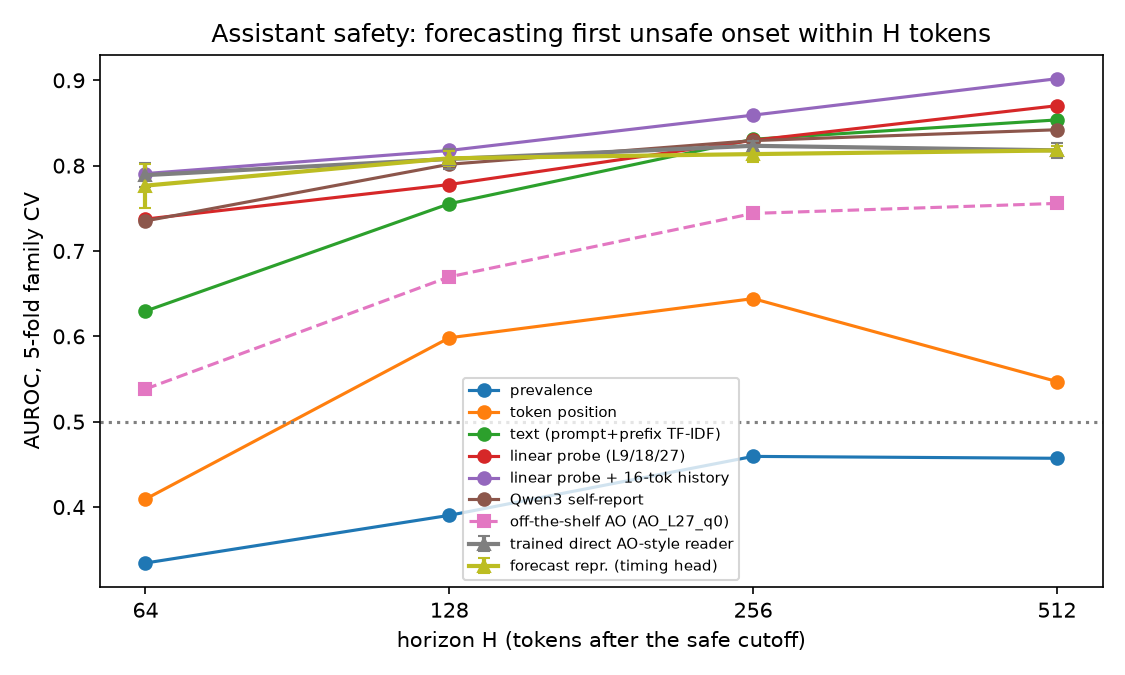
\includegraphics[width=0.85\linewidth]{figures/forecast_auroc_by_horizon_all.png}
\caption{{\bf \auroc by horizon} for the assistant setting (5-fold family CV). No informative method decays with lead distance; every method is weakest at $H{=}64$, where few positives exist and they must be separated from earlier prefixes of the same trajectory. \histprobe (purple) is best at every horizon. The off-the-shelf \ao (pink, dashed) is near chance at $H{=}64$. The \direct (gray) and \forecast (olive) readers nearly overlap and flatten at about 0.82.}
\label{fig:auroc}
\end{figure}

\begin{table}[t]
\centering
\caption{{\bf Forecasting the first unsafe onset within $H$ tokens} (assistant setting, safe prefixes only, 5-fold family CV, $n{=}3{,}520$ prefixes from 880 families). Cells give \auroc with 95\% family-bootstrap CIs. Trained readers give mean$\pm$sd over 3 seeds. \auprc and Brier are at $H{=}512$ (prevalence 10.7\%). Best in {\bf bold}. $^*$Out-of-fold constant predictions; values below 0.5 are a fold-composition artifact, not a signal.}
\label{tab:main}
\resizebox{\textwidth}{!}{%
\begin{tabular}{@{}llcccccc@{}}
\toprule
& & \multicolumn{4}{c}{\auroc at horizon $H$} & \multicolumn{2}{c}{$H{=}512$} \\
\cmidrule(lr){3-6} \cmidrule(lr){7-8}
& \textsc{Method} & $64$ & $128$ & $256$ & $512$ & \auprc$\uparrow$ & Brier$\downarrow$ \\
\midrule
\multirow{4}{*}{\rotatebox{90}{\scriptsize Baselines}}
& Prevalence$^*$ & 0.33 & 0.39 & 0.46 & 0.46 & 0.10 & 0.096 \\
& Token position & 0.41 {\scriptsize[.27,.56]} & 0.60 {\scriptsize[.49,.72]} & 0.64 {\scriptsize[.58,.70]} & 0.55 {\scriptsize[.52,.57]} & 0.12 & 0.095 \\
& \textprompt (prompt only) & 0.69 {\scriptsize[.55,.80]} & 0.72 {\scriptsize[.65,.79]} & 0.76 {\scriptsize[.70,.81]} & 0.77 {\scriptsize[.72,.81]} & 0.28 & 0.087 \\
& \textprefix (prompt+prefix) & 0.63 {\scriptsize[.47,.77]} & 0.76 {\scriptsize[.67,.84]} & 0.83 {\scriptsize[.78,.88]} & 0.85 {\scriptsize[.82,.89]} & 0.45 & 0.080 \\
\midrule
\multirow{4}{*}{\rotatebox{90}{\scriptsize Probes}}
& Linear probe L18 & 0.71 {\scriptsize[.60,.80]} & 0.78 {\scriptsize[.71,.85]} & 0.82 {\scriptsize[.78,.86]} & 0.87 {\scriptsize[.85,.89]} & 0.44 & 0.075 \\
& Linear probe L9+18+27 & 0.74 {\scriptsize[.63,.83]} & 0.78 {\scriptsize[.71,.85]} & 0.83 {\scriptsize[.79,.87]} & 0.87 {\scriptsize[.85,.89]} & 0.46 & 0.075 \\
& MLP probe L9+18+27 & 0.72 {\scriptsize[.62,.81]} & 0.76 {\scriptsize[.69,.83]} & 0.80 {\scriptsize[.76,.83]} & 0.84 {\scriptsize[.81,.87]} & 0.39 & 0.104 \\
& \histprobe (L18 + 16-token mean) & {\bf 0.79} {\scriptsize[.71,.87]} & {\bf 0.82} {\scriptsize[.75,.89]} & {\bf 0.86} {\scriptsize[.82,.90]} & {\bf 0.90} {\scriptsize[.88,.92]} & {\bf 0.50} & {\bf 0.071} \\
\midrule
\multirow{3}{*}{\rotatebox{90}{\scriptsize Verbal.}}
& \selfreport (\qwen) & 0.74 {\scriptsize[.66,.82]} & 0.80 {\scriptsize[.75,.85]} & 0.83 {\scriptsize[.79,.87]} & 0.84 {\scriptsize[.80,.88]} & 0.39 & 0.080 \\
& \ao, best (L27, q0) & 0.54 {\scriptsize[.44,.65]} & 0.67 {\scriptsize[.59,.75]} & 0.74 {\scriptsize[.70,.79]} & 0.76 {\scriptsize[.72,.79]} & -- & -- \\
& \ao (L18, q0) & 0.50 {\scriptsize[.39,.61]} & 0.63 {\scriptsize[.56,.70]} & 0.71 {\scriptsize[.67,.76]} & 0.75 {\scriptsize[.72,.78]} & -- & -- \\
\midrule
\multirow{2}{*}{\rotatebox{90}{\scriptsize Trained}}
& \direct reader (QA) & {\bf 0.79}{\scriptsize$\pm$.01} & 0.81{\scriptsize$\pm$.01} & 0.82{\scriptsize$\pm$.01} & 0.82{\scriptsize$\pm$.01} & 0.40 & 0.105 \\
& \forecast reader (timing head) & 0.78{\scriptsize$\pm$.02} & 0.81{\scriptsize$\pm$.01} & 0.81{\scriptsize$\pm$.01} & 0.82{\scriptsize$\pm$.01} & 0.37 & 0.108 \\
\bottomrule
\end{tabular}}
\end{table}


\subsection{How forecastable are delayed onsets?}
\label{sec:rq1}

\para{Activations forecast delayed onsets moderately well.}
\Tabref{tab:main} and \figref{fig:auroc} show the main results. A linear probe on all three layers reaches \auroc 0.74 at $H{=}64$ and 0.87 at $H{=}512$. \histprobe, which adds the mean of the last 16 layer-18 activations, is the best method at every horizon: 0.79, 0.82, 0.86, and 0.90. It also has the best \auprc (0.50 at 10.7\% prevalence) and the best Brier score (0.071).

\para{The hardest target is imminent onset, not distant onset.}
We expected \auroc to decay as the event moves further away. We find the opposite: every informative method has its \emph{lowest} \auroc at $H{=}64$. \auroc at $H$ is not a pure lead-distance curve, because the positive set changes with $H$. At $H{=}64$ the positives are prefixes 0--63 tokens before onset. Their negatives include earlier prefixes of the \emph{same} harmful trajectories, which look very similar. At $H{=}512$, by contrast, almost every prefix of a harmful trajectory is positive, so the task becomes ``is this a harmful request that \qwen will comply with?''

\para{Much of the long-horizon signal is visible in text.}
The prompt alone gives \auroc 0.77 at $H{=}512$, and the prompt+prefix text model reaches 0.85. Activations add the most at short horizons and with history: at $H{=}64$, \histprobe scores 0.79 vs.\ 0.63 for \textprefix, while at $H{=}512$ the gap shrinks to 0.90 vs.\ 0.85. Because the benign source has no events, request-level detection inflates long-horizon \auroc for every method equally. \textprompt is therefore the right yardstick for that shortcut, and \histprobe beats it at every horizon.

\para{The off-the-shelf Activation Oracle is the weakest non-trivial method.}
Zero-shot, the \ao answers ``Yes'' to only 0.6--1.1\% of prefixes for q0 and 12--15\% for q1. Even after 1-D calibration of its logit margin, its best variant (layer 27, q0) scores 0.54 at $H{=}64$, with a CI that includes chance, and 0.76 at $H{=}512$. This is below every probe, text model, and self-report score at every horizon. Layer 27 (75\% depth) is the AO's best read layer, as in its training. \selfreport, which also verbalizes but uses the target itself, does much better (0.74 to 0.84). It ties single-position probes but stays below \histprobe.

\subsection{Early warning}
\label{sec:ew}

\begin{table}[t]
\centering
\caption{{\bf Early warning at a target 5\% benign false-alarm rate.} We score with the $H{=}512$ output and set the threshold on benign validation families inside each training fold. Columns give the fraction of unsafe test trajectories whose first alert comes at least $k$ tokens before onset, and the realized test FAR. 88 unsafe and 792 benign trajectories (\ao: 78 and 670, from its own validation carve-out). Trained readers average 3 seeds. Best in {\bf bold}.}
\label{tab:ew}
\begin{tabular}{@{}lcccc@{}}
\toprule
\textsc{Method} & $\ge 64$ & $\ge 128$ & $\ge 256$ & Test FAR \\
\midrule
Prevalence / token position & 0.00 & 0.00 & 0.00 & 0.00 \\
\textprompt & 0.17 & 0.17 & 0.12 & 0.06 \\
\textprefix & 0.42 & 0.42 & 0.34 & 0.05 \\
Linear probe L9+18+27 & 0.42 & 0.42 & 0.31 & 0.04 \\
MLP probe L9+18+27 & 0.39 & 0.39 & 0.24 & 0.03 \\
\histprobe & {\bf 0.57} & {\bf 0.56} & {\bf 0.43} & 0.06 \\
\selfreport & 0.39 & 0.38 & 0.30 & 0.06 \\
\ao (L27, q0; best \auroc) & 0.22 & 0.22 & 0.13 & 0.05 \\
\ao (L18, q0; best alerts) & 0.36 & 0.36 & 0.27 & 0.06 \\
\direct reader & 0.38 & 0.37 & 0.22 & 0.04 \\
\forecast reader & 0.37 & 0.36 & 0.20 & 0.04 \\
\bottomrule
\end{tabular}
\end{table}


\begin{figure}[t]
\centering
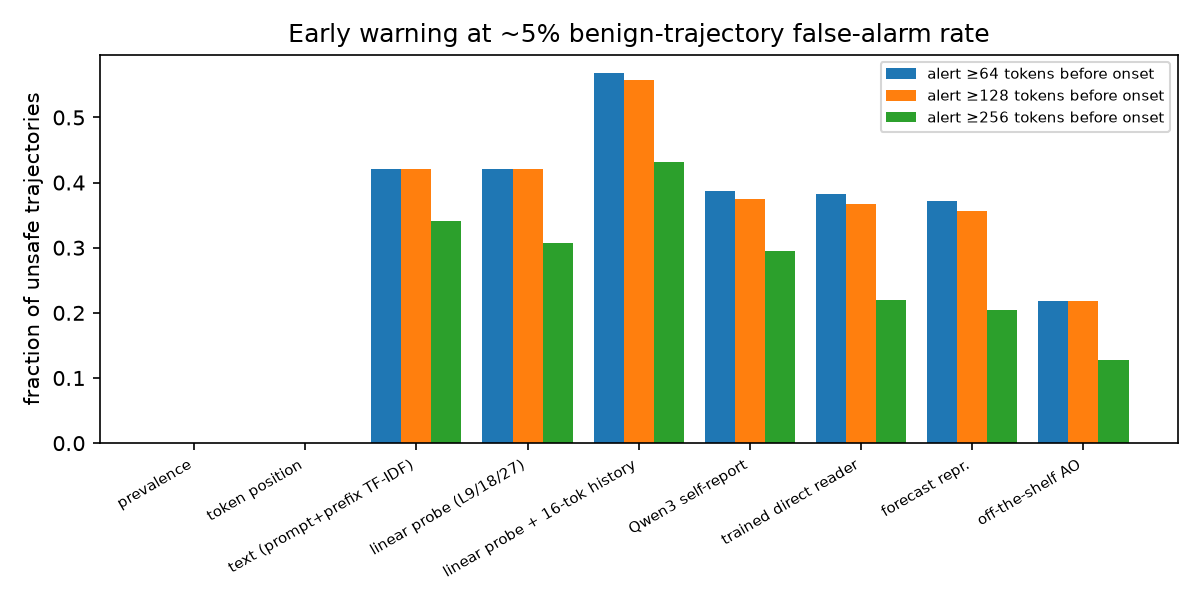
\includegraphics[width=0.85\linewidth]{figures/early_warning.png}
\caption{{\bf Early warning at about 5\% benign-trajectory false-alarm rate.} Bars show the fraction of unsafe trajectories alerted at least 64, 128, or 256 tokens before onset. \histprobe alerts on 56\% of trajectories at least 128 tokens ahead. The \ao bar shows the layer-27 q0 variant, which has the best \auroc but few alerts (22\%); the layer-18 q0 variant reaches 36\% (\tabref{tab:ew}).}
\label{fig:ew}
\end{figure}

\Tabref{tab:ew} and \figref{fig:ew} report the deployment-oriented metric. At a realized test FAR of 3--6\%, \histprobe alerts on 56\% of unsafe trajectories at least 128 tokens before onset. Single-position probes and \textprefix reach 42\%, \selfreport 38\%, and the trained readers 36--37\%. Prompt-only text reaches only 17\%, and prevalence and token position never alert. The $\ge$64 and $\ge$128 columns nearly coincide because onsets are late (median token 360) and alerts usually fire at the first cutoffs ($t{=}32$--$64$). When an alert happens, it is almost always far ahead; the main failure is \emph{missed} trajectories (40\% for \histprobe, 56\% for the linear probe). With 88 unsafe trajectories, the 95\% binomial interval around 0.37 is about $\pm$0.10, so the advantage of \histprobe over the trained readers (0.56 vs.\ 0.37) is about two standard errors.

\subsection{Does an explicit forecast representation help?}
\label{sec:rq2}

\begin{table}[t]
\centering
\caption{{\bf \forecast vs.\ matched \direct reader.} \auroc of seed-averaged out-of-fold predictions; $\Delta$ is the paired family-bootstrap difference with 95\% CI and two-sided $p$. Negative values favor \direct. Seed averaging (ensembling) gives higher \auroc than single seeds in \tabref{tab:main}.}
\label{tab:paired}
\resizebox{\textwidth}{!}{%
\begin{tabular}{@{}ccccll@{}}
\toprule
$H$ & \direct QA & \forecast head & \forecast QA & $\Delta$(head $-$ \direct) [CI], $p$ & $\Delta$(\forecast QA $-$ \direct) [CI], $p$ \\
\midrule
64  & {\bf 0.819} & 0.779 & 0.806 & $-0.040$ [$-0.093$, $0.005$], 0.10 & $-0.013$ [$-0.076$, $0.037$], 0.70 \\
128 & {\bf 0.844} & 0.826 & 0.811 & $-0.018$ [$-0.053$, $0.014$], 0.29 & $-0.034$ [$-0.081$, $0.010$], 0.13 \\
256 & {\bf 0.859} & 0.826 & 0.822 & $-0.033$ [$-0.056$, $-0.013$], 0.002 & $-0.038$ [$-0.062$, $-0.014$], $<$0.001 \\
512 & {\bf 0.851} & 0.833 & 0.821 & $-0.018$ [$-0.034$, $-0.003$], 0.014 & $-0.031$ [$-0.053$, $-0.011$], $<$0.001 \\
\bottomrule
\end{tabular}}
\end{table}


\para{The forecast representation does not beat the direct reader.}
\Tabref{tab:paired} compares seed-averaged out-of-fold predictions. The \forecast timing head trails \direct at every horizon: $\Delta$\auroc $=-0.040$, $-0.018$, $-0.033$, and $-0.018$ for $H=64$ to $512$. The difference is significant at $H{=}256$ ($p{=}0.002$) and $H{=}512$ ($p{=}0.014$) and not significant at $H\le128$. Reading answers from the forecast vectors through the shared QA head does not help either: it is significantly worse than \direct at $H\ge256$ ($p<0.001$). Early warning tells the same story: 36\% vs.\ 37\% of unsafe trajectories alerted at least 128 tokens ahead (\tabref{tab:ew}). An earlier run of the same code under a different software stack gave the same ordering (\appref{app:details}).

\begin{table}[t]
\centering
\caption{{\bf Ablations, controls, and question generalization} (QA \auroc; single seed for ablations/controls, mean$\pm$sd over 3 seeds for the main readers). ``Refuse later'' is never trained. The gold-readout row feeds true future bins to the \forecast QA head and is an upper bound on readout, not a forecaster.}
\label{tab:controls}
\resizebox{\textwidth}{!}{%
\begin{tabular}{@{}lccccccc@{}}
\toprule
& \multicolumn{4}{c}{Occurrence within $H$} & \multicolumn{2}{c}{Other trained questions} & Held-out \\
\cmidrule(lr){2-5} \cmidrule(lr){6-7} \cmidrule(lr){8-8}
\textsc{Model} & 64 & 128 & 256 & 512 & Harm.\ rec.\ 512 & Topic chg.\ 128 & Refuse later \\
\midrule
\direct & {\bf 0.79}{\scriptsize$\pm$.01} & {\bf 0.81}{\scriptsize$\pm$.01} & {\bf 0.82}{\scriptsize$\pm$.01} & {\bf 0.82}{\scriptsize$\pm$.01} & {\bf 0.82}{\scriptsize$\pm$.01} & {\bf 0.70}{\scriptsize$\pm$.00} & {\bf 0.63}{\scriptsize$\pm$.01} \\
\forecast & 0.78{\scriptsize$\pm$.02} & 0.79{\scriptsize$\pm$.01} & 0.80{\scriptsize$\pm$.01} & 0.79{\scriptsize$\pm$.00} & 0.79{\scriptsize$\pm$.01} & 0.67{\scriptsize$\pm$.00} & 0.57{\scriptsize$\pm$.02} \\
\forecast + raw-activation bypass & 0.75 & 0.78 & 0.80 & 0.80 & 0.80 & 0.69 & 0.59 \\
\midrule
\direct, shuffled activations & 0.31 & 0.47 & 0.47 & 0.48 & 0.48 & 0.57 & 0.49 \\
\forecast, shuffled activations & 0.43 & 0.52 & 0.51 & 0.48 & 0.49 & 0.58 & 0.49 \\
\direct, constant activation & 0.38 & 0.57 & 0.60 & 0.54 & 0.56 & 0.65 & 0.49 \\
\forecast, constant activation & 0.38 & 0.57 & 0.60 & 0.54 & 0.56 & 0.65 & 0.48 \\
\midrule
\forecast, gold future bins (ceiling) & 0.75 & 0.78 & 0.84 & 0.96 & 0.97 & 0.67 & 0.58 \\
\bottomrule
\end{tabular}}
\end{table}


\para{Controls rule out shortcut explanations.}
\Tabref{tab:controls} shows the ablations and controls. With shuffled activations, \auroc falls to 0.31--0.52 and only 3\% of unsafe trajectories are alerted early. With a constant mean activation, so that only position information remains, \auroc is 0.38--0.62 and there are no alerts. Adding a raw-activation bypass to \forecast does not help (0.78 and 0.80 at $H{=}128$ and $512$). The trained readers therefore rely on activation content, not on position or prompt-level artifacts in the training pipeline.

\para{The bottleneck is the forecast, not the readout.}
When we feed the \emph{gold} future bins to the \forecast QA head, it reaches 0.96 for occurrence within 512 and 0.97 for harmful recommendation within 512. The head can decode answers from a correct forecast. It stays weaker for the rare short-horizon questions (0.75 at 64 and 0.78 at 128), where a small head with positive weight 3 underfits classes at 1--2\% prevalence. The \forecast model falls short because its predicted forecast is no better than what an unconstrained reader learns directly.

\subsection{Further analyses}
\label{sec:extra}

\para{One representation, several questions.}
Both readers answer all trained questions from a single representation (\tabref{tab:controls}). \direct leads on harmful recommendation within 512 (0.82 vs.\ 0.79) and topic change within 128 (0.70 vs.\ 0.67). On the held-out question meaning, ``will the assistant refuse or back away later'', both are only weakly above chance, and \forecast generalizes worse (0.57$\pm$0.02 vs.\ 0.63$\pm$0.01). Behavior-type questions are nearly redundant with occurrence here, because 93 of 95 events are harmful recommendations.

\para{Activation history is the most useful addition.}
\begin{table}[t]
\centering
\caption{{\bf Effect of a 16-token activation history} on the layer-18 linear probe (\auroc, and fraction of unsafe trajectories alerted $\ge$128 tokens before onset at about 5\% FAR).}
\label{tab:history}
\begin{tabular}{@{}lccccc@{}}
\toprule
\textsc{Probe input} & $H{=}64$ & $H{=}128$ & $H{=}256$ & $H{=}512$ & Alert $\ge$128 \\
\midrule
Last token only & 0.71 & 0.78 & 0.82 & 0.87 & 0.41 \\
+ 16-token mean & {\bf 0.79} \increase & {\bf 0.82} \increase & {\bf 0.86} \increase & {\bf 0.90} \increase & {\bf 0.56} \increase \\
\bottomrule
\end{tabular}
\end{table}
\Tabref{tab:history} isolates the history effect. Averaging the last 16 layer-18 activations improves \auroc by 0.08 at $H{=}64$ and 0.03 at $H{=}512$, and it raises early alerts from 41\% to 56\%. This one change matters more than any other modeling choice in our study, including the trained readers, which see only the last position.

\para{Story setting.}
\Tabref{tab:story} reports the fictional-harm setting, where the event is the first fictional-harm description in a story. Here, \emph{whether} harm happens is mostly fixed by the prompt: \textprompt reaches 0.84 at $H{=}512$, above \histprobe (0.81). Activations help at short horizons, \ie with \emph{when} the scene starts: \histprobe scores 0.79 at $H{=}64$ vs.\ 0.67 for \textprompt. \selfreport is poor (0.57--0.66), because \qwen does not consider fiction ``harmful content''. This matches our rubric, which does not treat fiction as an assistant violation. The \ao does relatively better here (0.66--0.73) than in the assistant setting.

\begin{table}[t]
\centering
\caption{{\bf Story setting} (event = first fictional-harm description; 439 safe prefixes, 96 families; prevalence 7.5\% at $H{=}64$ to 64\% at $H{=}512$). \auroc, 5-fold family CV. Best in {\bf bold}.}
\label{tab:story}
\begin{tabular}{@{}lcccc@{}}
\toprule
\textsc{Method} & $64$ & $128$ & $256$ & $512$ \\
\midrule
Token position & 0.64 & 0.65 & 0.56 & 0.44 \\
\textprompt & 0.67 & 0.71 & {\bf 0.72} & {\bf 0.84} \\
\textprefix & 0.71 & 0.71 & 0.71 & {\bf 0.84} \\
\histprobe & {\bf 0.79} & {\bf 0.79} & 0.71 & 0.81 \\
\selfreport & 0.57 & 0.59 & 0.61 & 0.66 \\
\ao (L27, q0) & 0.70 & 0.66 & 0.69 & 0.72 \\
\ao (L18, q1) & 0.73 & 0.71 & 0.69 & 0.67 \\
\bottomrule
\end{tabular}
\end{table}


\para{Detection is easier than forecasting.}
For comparison, a linear probe on all three layers separates already-unsafe prefixes from safe ones with \auroc 0.86 [0.79, 0.91] (71 positive prefixes from 22 families). This is above every forecaster at $H{=}64$.

\section{Discussion}
\label{sec:discussion}

\para{What do the activations know about a coming violation?}
Our results suggest two kinds of signal. The first is request-level: which request this is and whether \qwen has started to comply. This signal dominates at long horizons, and text sees much of it (prompt-only \auroc 0.77 and prompt+prefix 0.85 at $H{=}512$). The second is local and concerns \emph{when} the response turns. It matters most at short horizons, where text fails (0.63 at $H{=}64$) and activations, especially averaged over a short history, do much better (0.79). The story setting shows the same split: the prompt decides whether a violent scene happens, while activations help predict when it starts. This fits the ``breadcrumbs'' view of \citet{wu2024planahead}: the model carries features that are useful for the current text and also predict the future, rather than an explicit plan with a timestamp.

\para{Why do zero-shot verbalizers fail here?}
The off-the-shelf \ao answers ``No'' to about 99\% of prefixes on the main question. Its calibrated margin is near chance for imminent onsets. This matches the ``safe'' prior that both \citet{bauer2026building} and our own LatentQA smoke test observed. The \ao was trained on current-state questions and on predicting the next few tokens, so a question about harm hundreds of tokens away is far outside its training distribution. Training on future-event labels fixes most of the gap: the AO-style \direct reader improves on the \ao by 0.25 \auroc at $H{=}64$ (0.79 vs.\ 0.54). Even so, the trained readers do not beat a linear probe with history.

\para{Supervision, not architecture.}
Our main hypothesis was that an explicit future representation (horizon queries, forecast vectors, and a timing head) would help beyond a direct reader trained on the same labels. The data do not support it. \forecast ties \direct at $H\le128$ and loses slightly at $H\ge256$. It also generalizes worse to the held-out question meaning. The readout-ceiling diagnostic locates the problem: the QA head can use a correct forecast (0.96 at $H{=}512$), but the predicted forecast is not better than what an unconstrained reader learns. With only 88 positive families, a 5-bin hazard bottleneck is probably data-starved. The bottleneck could still help with many more positive families, with a semantic auxiliary loss, or with an LLM decoder that benefits from a compact structured input. We did not test these settings.

\para{Practical implications.}
For early warning of delayed harm, a linear probe on a short activation history, together with the prompt, is the baseline to beat. It is cheap and it outperformed every verbalizer and trained reader we tested. Zero-shot verbalizers asked yes/no safety questions should not be trusted as forecasters without calibration and a probe comparison. Because most missed trajectories are never alerted at all, improving recall at a fixed FAR matters more than improving lead time.

\para{Limitations.}
\begin{itemize}[leftmargin=*,itemsep=0pt,topsep=0pt]
    \item \textbf{Few events.} There are 88 assistant event families and only 22 at $H{=}64$, so CIs are wide. The fixed test split has 2--8 positive families, so we report 5-fold family CV with hyperparameters fixed in advance.
    \item \textbf{LLM labels without a human check.} Inter-annotator $\kappa$ is 0.69, the primary annotator is more liberal than the second one, and onsets agree within 32 tokens only 70\% of the time. This mostly blurs the $H{=}64$ labels.
    \item \textbf{Single rollouts.} Each family has one sample from a stochastic policy, so labels are single realizations. We did not run repeated-rollout calibration of the label noise.
    \item \textbf{Lightweight readers.} Our \direct and \forecast readers are small attention heads on cached activations, not pretrained LLM decoders with LoRA, and they omit the semantic auxiliary loss. Our conclusions about architecture hold for this reader family only.
    \item \textbf{Limited verbalizer coverage.} We test one AO checkpoint with a single injected position, two questions, and yes/no scoring. Multi-position or open-ended querying may do better. We did not evaluate LatentQA or other decoders on \qwen activations because no compatible checkpoint exists.
    \item \textbf{Scope.} We study one target model in non-thinking mode with natural onsets. We did not build model organisms with controlled delays, so we cannot separate plan-like signals from position effects in harmful trajectories.
    \item \textbf{Software drift.} The analysis environment changed between generation and analysis (\appref{app:details}). Generation was unaffected, and the \direct-vs-\forecast ordering replicated across versions.
\end{itemize}

\para{Broader impact.}
Forecasting monitors could stop harmful content before it is emitted, which is the main motivation for this work. The same forecasts could also be used adversarially, for example to search for prompts that delay harm past a monitor's horizon. We release no new harmful content. Our generations and annotations contain harmful text from the target model and should be shared only under access controls.

\section{Conclusion}
\label{sec:conclusion}

We asked whether a still-safe prefix of a \qwen response reveals that a clear safety violation is coming within the next 64--512 tokens. On a family-split benchmark of natural generations, it partly does. A linear probe on a 16-token activation history reaches \auroc 0.79 at 64 tokens and 0.90 at 512 tokens, and it flags 56\% of unsafe trajectories at least 128 tokens before onset at a 5\% benign false-alarm rate. An off-the-shelf Activation Oracle does poorly zero-shot. Training on future-event labels closes most of that gap, but an explicit forecast representation adds nothing over a matched direct reader. The key takeaway is that future-event supervision, not forecast architecture, drives the gains, and that a cheap activation-history probe is the baseline any verbalizer-based forecaster must beat.

Future work should scale the number of positive families with more rollouts per harmful prompt, and calibrate labels with repeated rollouts. Windowed or recurrent encoders could exploit the history signal in both the direct and forecast readers. The most direct next test is an LLM-decoder AO fine-tuned on these future-event labels, with and without the forecast bottleneck. Model organisms with controlled delays, compared against a token-position control, would show whether the history signal reflects plans or position.


\bibliography{references}

\appendix
\section{Additional Experimental Details}
\label{app:details}

\para{Data sources and splits.}
\Tabref{tab:sources} lists the prompt sources. Families were split 80/10/10 per source with a fixed seed before generation. Each family appears in exactly one split and one cross-validation fold, and we assert this in code.

\begin{table}[h]
\centering
\caption{Prompt families after annotation (987 of 1,000; 13 annotator calls failed).}
\label{tab:sources}
\resizebox{\textwidth}{!}{%
\begin{tabular}{@{}lccl@{}}
\toprule
\textsc{Source} & Families & Event rate & Role \\
\midrule
Harmful long-form (HarmBench / AdvBench / StrongREJECT) & 408 & 15.9\% & assistant \\
Gray long-form (BeaverTails unsafe questions) & 200 & 15.0\% & assistant \\
Benign long-form (Alpaca) & 279 & 0\% & assistant (matched negatives) \\
Story prompts & 100 & 72\% (fictional harm) & reported separately \\
\bottomrule
\end{tabular}}
\end{table}

\para{Onset distribution.}
Among the 88 assistant event families, onset quantiles are 79 (10\%), 273 (25\%), 360 (50\%), 483 (75\%), and 557 (90\%) response tokens.

\para{Annotation check.}
The second annotator (\texttt{gpt-5.6-terra}) re-labeled 200 generations stratified so that half were flagged by the primary annotator. Event agreement was 84.5\% ($\kappa{=}0.69$), and fiction-label agreement was 99\%. The second annotator confirmed 68\% of primary flags and flagged nothing the primary annotator missed. The median onset difference was 1 token, and 70\% of onsets agreed within 32 tokens.

\para{Calibration of verbal scores.}
For \selfreport and the \ao we use the Yes$-$No logit margin of the next token as a score. We fit a 1-D logistic calibration inside each training fold. Calibration does not change \auroc within a fold but makes pooled out-of-fold scores comparable across folds.

\para{Trained readers.}
Both readers use AdamW (learning rate $3{\times}10^{-4}$), 30 epochs, batch size 128, positive weight 3 on QA losses, and seeds 0--2. The \forecast timing head has five bins (onset within 64, 128, 256, 512 tokens, or later/never) and predicts discrete hazards. Censored horizons would be masked in the likelihood, although none occur in our data.

\para{Replication across software versions.}
Generation used torch 2.7.1. Extraction, the main E2 run, and the AO evaluation used torch 2.14.1 and transformers 5.20, because upgrading peft to load the AO pulled in a newer torch. An earlier E2 run of the same code under torch 2.7.1 gave the same ordering: \direct 0.817$\pm$0.004 vs.\ \forecast head 0.814$\pm$0.003 \auroc at $H{=}512$, and 37\% vs.\ 33\% of unsafe trajectories alerted at least 128 tokens ahead.

\para{Compute and cost.}
All model computation ran on one NVIDIA RTX A6000 (48\,GB). Annotation used about 1,200 API calls and question embedding 7 calls, at a total cost of a few US dollars.


\end{document}
